
%%%%%%%%%%%%%%%%%%%%%%%%%%%% PACKAGES %%%%%%%%%%%%%%%%%%%%%%%%%%%%%%%%%%%
% Layout
\documentclass{article}
\usepackage[utf8]{inputenc}
\usepackage{geometry}
\geometry{a4paper,left=30mm,right=30mm,top=30mm,bottom=30mm}
\usepackage{rotating}
\usepackage{pdflscape}

%%%%%%% Two columns %%%%%%%%
% \documentclass[twocolumn]{article}
% \setlength{\columnsep}{10mm}

% Various
\usepackage[colorinlistoftodos]{todonotes}
\usepackage{hyperref}
\usepackage{siunitx} % for symbols like °
\usepackage{amsmath}
\newcommand\pro{\item[$+$]}
\newcommand\con{\item[$-$]}

% Images
\usepackage{graphicx}
\graphicspath{ {Images/} }
\usepackage{subfigure}
\usepackage{wrapfig}

% Tables 
\usepackage{booktabs}

% Titlepage
\usepackage[affil-it]{authblk}
\usepackage{fancyhdr}


%%%%%%%%%%%%%%%%%%%%%%%%%%%% DOCUMENT %%%%%%%%%%%%%%%%%%%%%%%%%%%%%%%%%%%
\begin{document}


%%%%%%%%% Title Page %%%%%%%%%

\begin{titlepage}

\newcommand{\HRule}{\rule{\linewidth}{0.5mm}} % Defines a new command for the horizontal lines, change thickness here
\begin{center}{
\HRule \\[0.4cm] 
\huge \bfseries{System design of a geothermal sourced CO2 network in a residential district}
\HRule \\[0.5cm]}
\end{center}

% To add title
\title{Master thesis at IPESE, Sion}

% To add the authors
\author[2]{Tobia Wyss\thanks{tobia.wyss@epfl.ch}}

\author[1]{Amorim Leandro De Castro Amoedo Rafael \thanks{rafael.amoedo@epfl.ch}}
\author[1]{Luc Girardin\thanks{luc.girardin@epfl.ch}}
\author[1]{Fran\c{c}ois Mar\'echal\thanks{francois.marechal@epfl.ch}}

%To add the affiliations
\affil[1]{Industrial Process and Energy Systems Engineering (IPESE), EPFL}
\affil[2]{Master Student, Energy Management and Sustainability , EPFL}



%% To set the bibliography style
%\bibliographystyle{unsrt} %other styles: https://www.sharelatex.com/learn/Bibtex_bibliography_styles
%\bibliography{bibliography}

\date{\today} %add date if you want to display it in the cover page
{\let\newpage\relax\maketitle}
\vspace*{\fill}

% To add the logos
\begin{figure*}[!htb]
\centering
\subfigure{
\includegraphics[width=4cm]{Logos/logo_epfl.eps}}\hfill
\quad
\subfigure{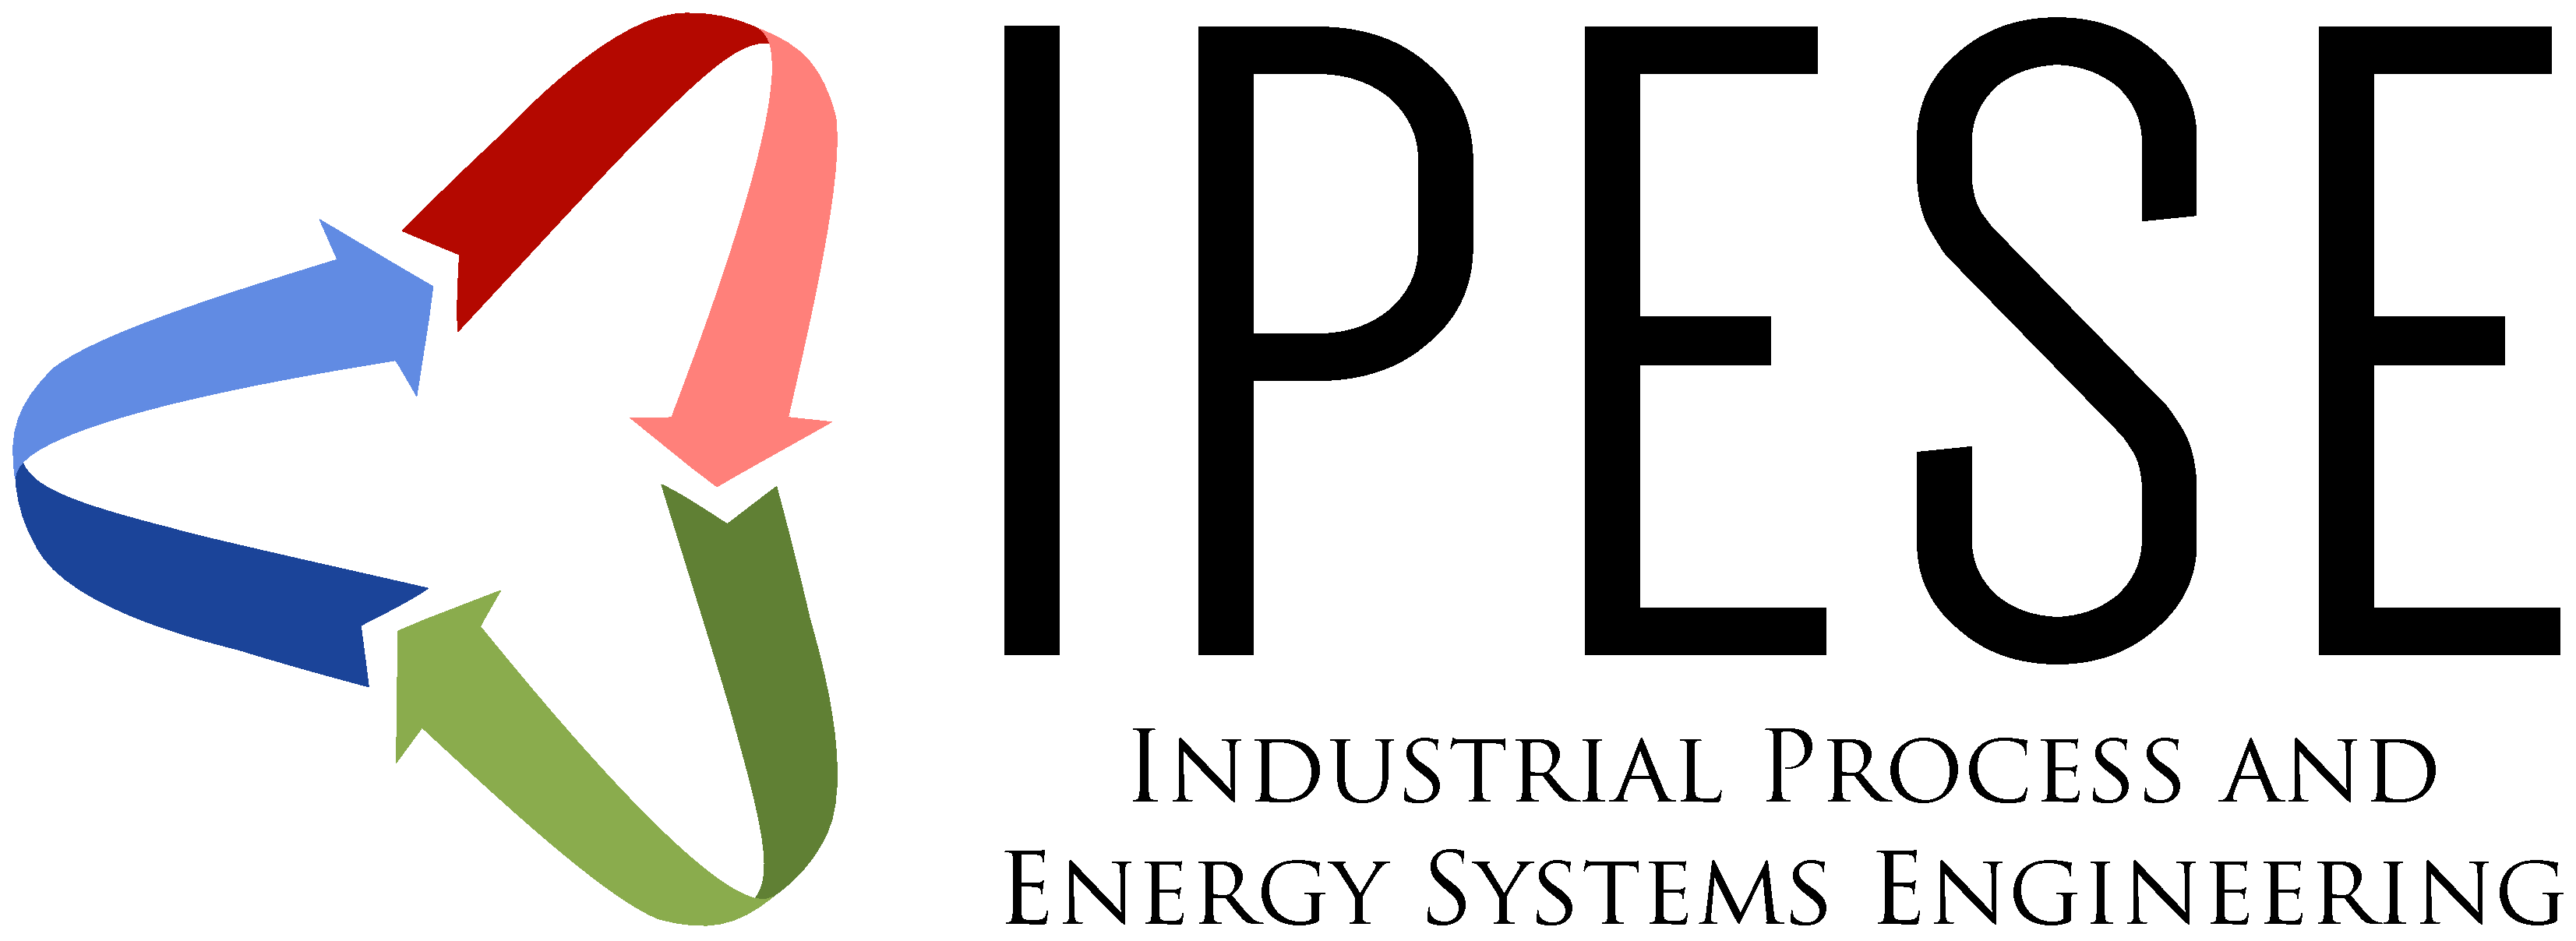
\includegraphics[width=4.6cm]{Logos/logo_ipese.eps}}
\end{figure*}

% To add footnote to the title page
\fancypagestyle{postprintnote}{\fancyhf{}\renewcommand{\headrulewidth}{0pt}\fancyfoot[R]{%
%footer text goes here
}}
\thispagestyle{postprintnote}

\end{titlepage}


% \begin{titlepage}

% \newcommand{\HRule}{\rule{\linewidth}{0.5mm}} % Defines a new command for the horizontal lines, change thickness here

% \center % Center everything on the page
% %----------------------------------------------------------------------------------------
% %	TITLE SECTION
% %----------------------------------------------------------------------------------------

% \HRule \\[0.4cm]
% { \huge \bfseries CO2 Networks}\\[0.4cm] % Title of your document
% { \Large \bfseries --- A Case Study ---}\\[0.4cm] % Title of your document
% \HRule \\[1.5cm]
 
% %----------------------------------------------------------------------------------------
% %	AUTHOR SECTION
% %----------------------------------------------------------------------------------------

% \begin{minipage}{0.4\textwidth}
% \begin{flushleft} \large
% \emph{Authors:}\\
% Tobia \textsc{Wyss} 
% \author[2]{Tobia Wyss\thanks{tobia.wyss@epfl.ch}}
% \end{flushleft}
% \end{minipage}

% ~
% \begin{minipage}{0.4\textwidth}
% \begin{flushright} \large
% \emph{Supervisors:} \\
% Pr. François \textsc{MARECHAL}\\
% \author[1]{Fran\c{c}ois Mar\'echal\thanks{francois.marechal@epfl.ch}}
% Luc  \textsc{GIRARDIN}\\
% Luise \textsc{MIDDELHAUVE}

% \end{flushright}
% \end{minipage}\\[2cm]

% %To add the affiliations
% \affil[1]{Industrial Process and Energy Systems Engineering (IPESE), \'Ecole Polytechnique F\'ed\'erale de Lausanne}
% \affil[2]{Master student, \'Ecole Polytechnique F\'ed\'erale de Lausanne}

% %----------------------------------------------------------------------------------------
% %	LOGO SECTION
% %----------------------------------------------------------------------------------------

% % To add the logos
% \begin{figure*}[!htb]
% \centering
% \subfigure{
\includegraphics[width=4cm]{Logos/logo_epfl.eps}}\hfill
% \quad
% \subfigure{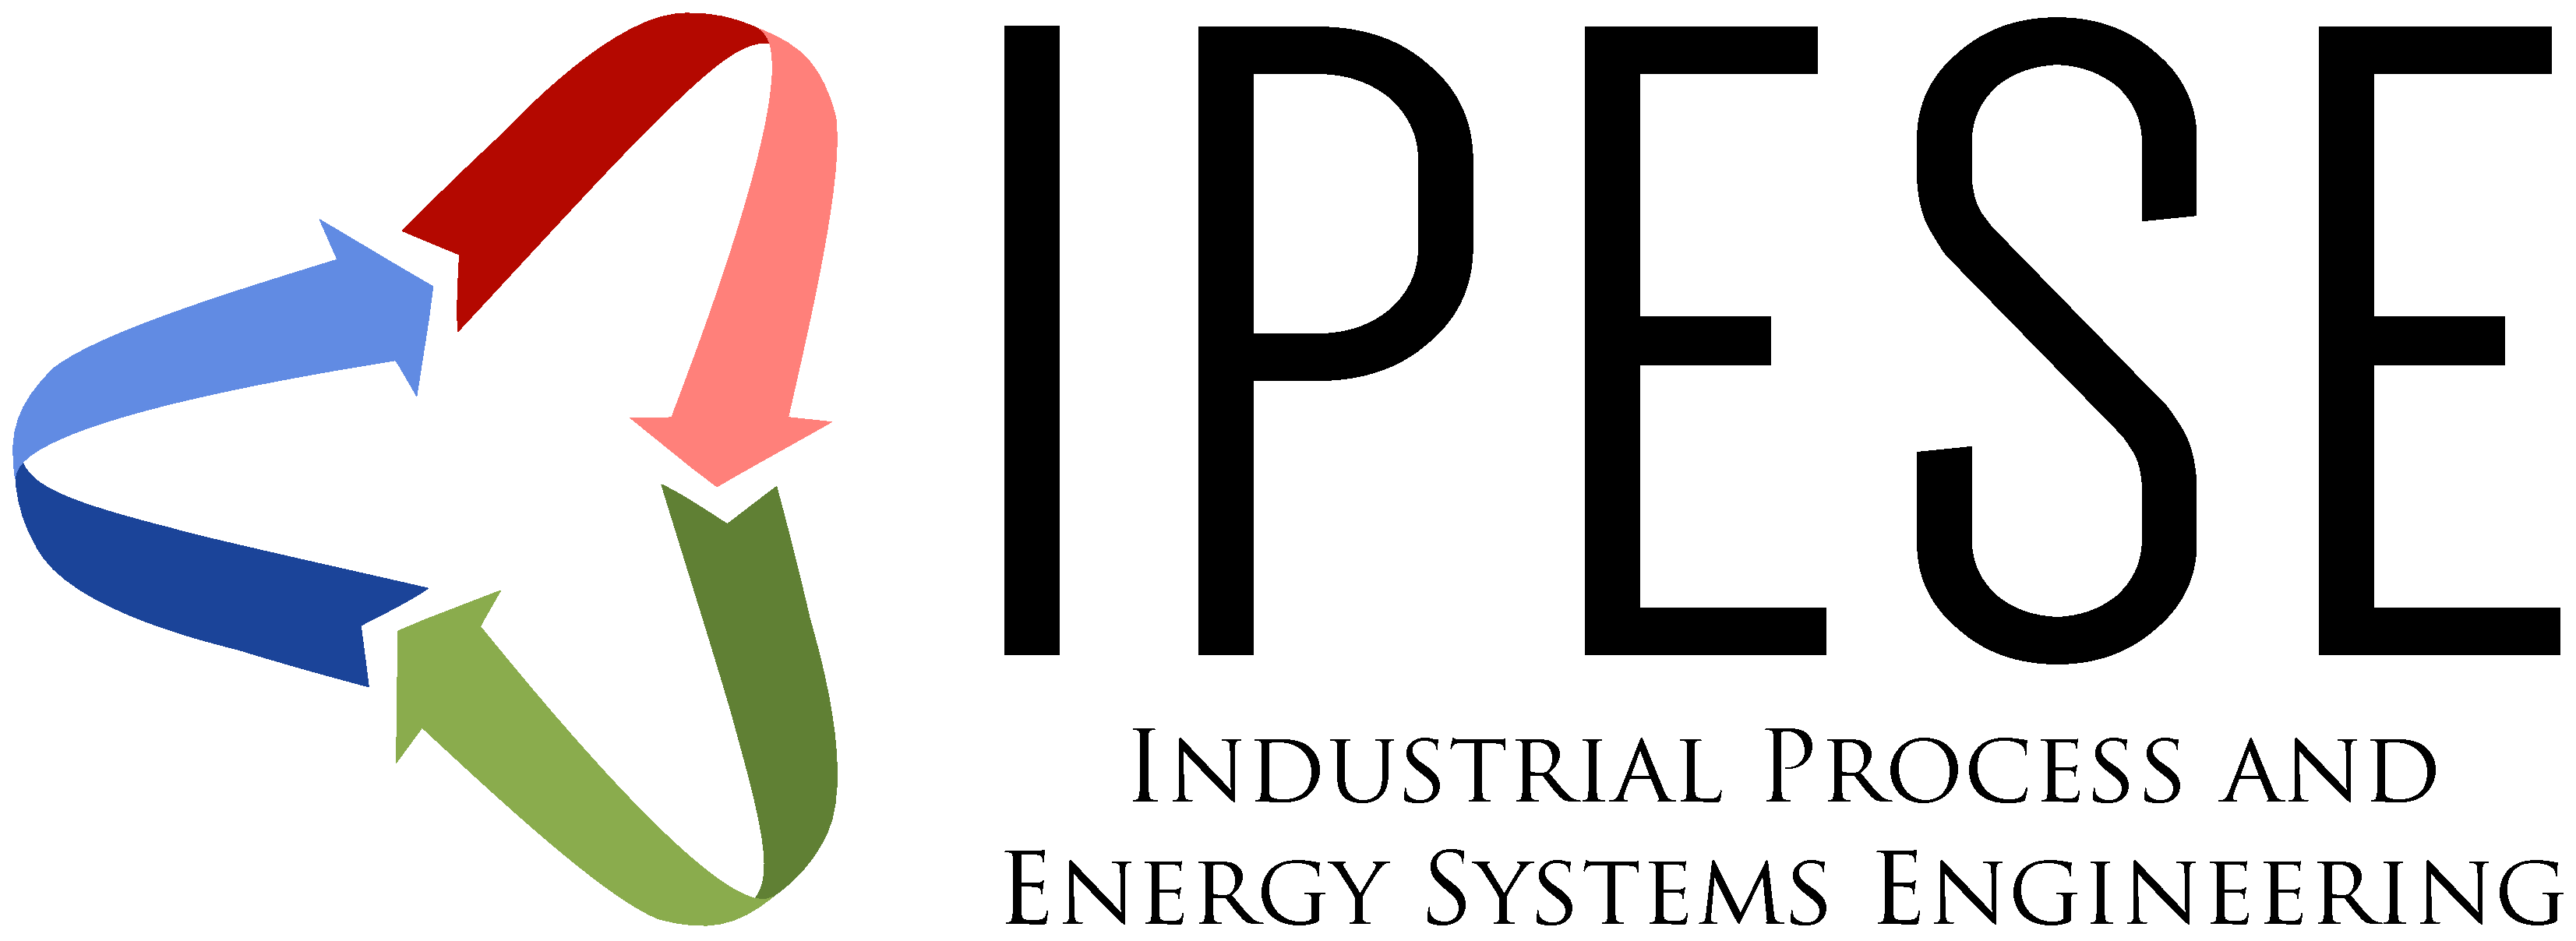
\includegraphics[width=4.6cm]{Logos/logo_ipese.eps}}
% \end{figure*}

% {\let\newpage\relax\maketitle}
% % To add footnote to the title page
% \fancypagestyle{postprintnote}{\fancyhf{}\renewcommand{\headrulewidth}{0pt}\fancyfoot[R]{%
% %footer text goes here
% }}
% \thispagestyle{postprintnote}

% \thispagestyle{empty}
% \clearpage

% \end{titlepage}


%%%%%%%%% Empty page %%%%%%%%%
\newpage
\null
\thispagestyle{empty} % to have a page without page number
\clearpage

%%%%%%%%% TODOS %%%%%%%%%
\listoftodos
\newpage

%%%%%%%%% Contents %%%%%%%%%
\begin{abstract}
District energy systems present a high potential to reduce CO2 emissions caused by cities, thanks to the implementation of large polygeneration energy conversion technologies connected to buildings over a network.
A specific technology, developed by EPFL, using a CO2 network...
A comparative analysis shows that...
\end{abstract}

%%%%%%%%% Contents %%%%%%%%%
\newpage
\tableofcontents
\thispagestyle{empty} 

%%%%%%%%% List of Figures %%%%%%%%%
%\newpage
%\listoffigures
%\thispagestyle{empty}

%%%%%%%%% List of Tables %%%%%%%%%
%\newpage
%\listoftables
%\thispagestyle{empty}


%%%%%%%%% Reset page counter %%%%%%%%%
\setcounter{page}{1}
\renewcommand{\thepage}{\arabic{page}}
\newpage

%%%%%%%%%%%%%%%%%%%%%%%%%%%% CONTENT %%%%%%%%%%%%%%%%%%%%%%%%%%%%%%%%%%%
\section*{Glossary}
SH
DHW
REF
AC
GC
CP
ERA
PV
HP
GSHP
SL-
DX-
SIA
PV
DEN
HEX
DH
DHC
CHP
is
mech
comp
ex
evap 
cond
MILP
PtG
DSM
HFC
HCFC
CFC
HFO
IC
OC
TC
CAPEX
OPEX

\section{Introduction}

\subsection{Context}
Throughout the last decades, human society has developed thanks to energy, most of which has come from fossil fuels. This has led to an unprecedented rise in CO2 emissions, which have proved to be at the source of climate change. In order to secure a livable planet for the years to come, it is necessary, among others, to drastically reduce CO2 emissions\cite{ipccSummaryPolicymakersIPCC2018}. Since the adoption of the Kyoto protocol, the first international treaty about the fight against climate change in 1992, many countries have agreed to drastically reduce CO2 emissions in the coming decades.\\

One crucial sector is the production of heat, which represents a large share of the total greenhouse emissions. This is especially true for countries at higher latitudes, i.e. with cold climates. For example in Switzerland the energy demand for space heating and hot water demand of buildings, accounts for around 41\% (96.5 TWh) of the total energy demand of the country, and is still strongly dependent from fossil fuels. If we also include process heat, this figure rises to 54\% (123.9 TWh)\cite{bacherEnergieRespektSchlusselFur2014}. 

Also the energy demand related to cooling is experiencing an exponential growth. This is, on the one hand, because it is becoming affordable for more people, as income levels rise. On the other hand, this increase is due to global warming, which leads worldwide to a higher average temperature, as well as an increase in the frequency of days with extreme temperatures\cite{ipccSummaryPolicymakersIPCC2018}. There are today 1.6 billion air conditioners (AC) in use, and about 50\% of them are distributed in only two countries: China and USA. In some countries, especially in the Middle East, as well as in parts of the USA, during extremely hot days cooling can represent more than 70\% of peak residential electricity demand. A huge problem with respect to this, is the quality of ACs. The majority of ACs that are sold in large markets, have an efficiency, which is only 50\% or lower than the one of the best products available. This engenders, obviously, an important augmentation of the energy demand. Figure \ref{fig:cooling_energy} shows how the energy demand has tripled since 1990, while the share of cooling energy in total energy use in buildings has risen from 2\% to more almost 7\% \cite{birolFutureCooling2018}. 

\begin{figure}[h!]
	\centering
	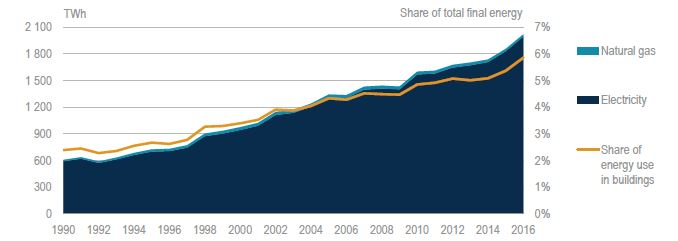
\includegraphics[width=0.7\textwidth]{cooling_energy.JPG}
	\caption{World energy consumption for space cooling in buildings. Source:\cite{birolFutureCooling2018}}
	\label{fig:cooling_energy}
\end{figure}

A study shows that also in Switzerland cooling demand will strongly increase in the next decades, due to climate change. Figure \ref{fig:climat_CH} shows how this is particularly true for modern houses, which are very well isolated and efficient for the winter use. In this case the cooling demand will represent more or less a third of the heating demand\cite{hsluClimaBauPlanenAngesichts2017}.\\

\begin{figure}[h!]
	\centering
	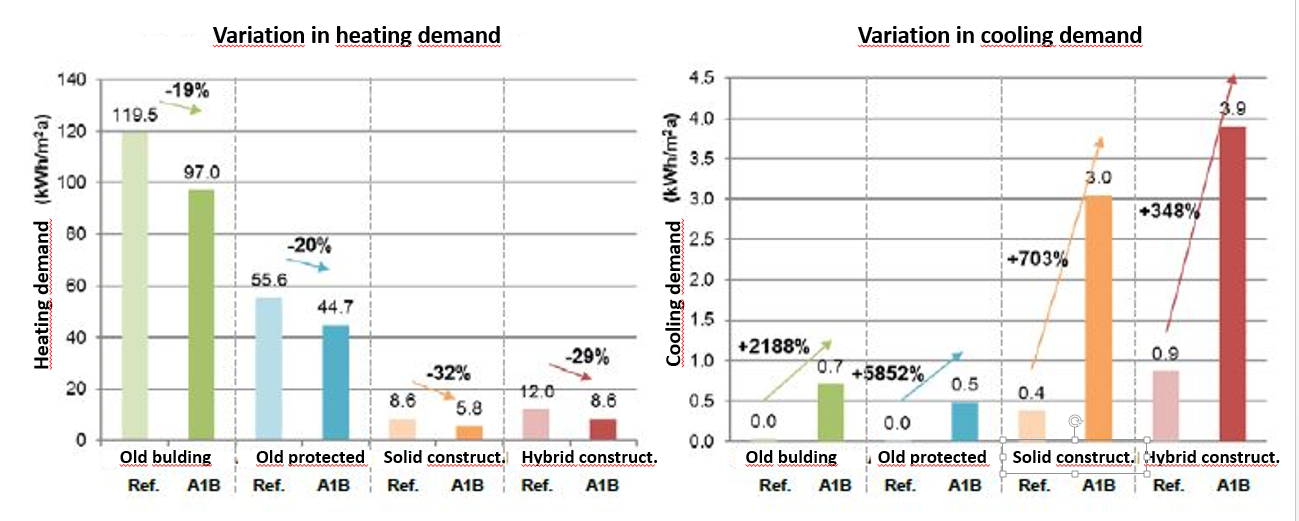
\includegraphics[width=0.7\textwidth]{clima_CH.png}
	\caption{The evolution of median values of heating (left) and cooling (right) demand of the fours case studies ("Old building", "Old builing protected", "Solid construction", "Hybrid construction") between the reference period "1995" (1980-2009) and the period "2060" (2045-2074) in Basel. The percentage variations can be attributed to climate change. A1B corresponds to a median scenario developed by the IPCC. Source: \cite{hsluClimaBauPlanenAngesichts2017}}
	\label{fig:climat_CH}
\end{figure}

According to the Population Division of the United Nations, the share of the world population living in cities has steadily increased from 34\% in 1960 to 55\% in 2017. Moreover, they prospect that, by 2050, this number will rise to 66\%. In Switzerland, as well as in its neighbouring countries, the percentage of urban population is considerably higher, with 74\% (2017) \cite{unitednationspopulationdivisionWorldUrbanizationProspects}.
The fact that people live more and more in concentrated areas, also mean that the density of energy consumption is rising. This becomes particularly interesting for urban heating and cooling demand, since the high density of heat consumers sets the conditions for efficient  systems, based on district energy networks. 

The UNEP (United Nations Environment Programme) has identified a big potential in modern district energy systems, as the most effective approach to improve energy efficiency for heating and cooling, and enable the integration of renewable energies. However, these technologies require a high level of technology coordination and planning, since they create more efficient systems that are also more complex to deploy and operate. This is why, further research and technology development are needed in order to foster the spreading of these technologies.

% \textit{Generally, these networks rely on centralized energy conversion technologies supplying heating and/or cooling to the users through a water network. In most of the cases, the supply temperature of these networks is selected, at best, according to the most demanding consumer connected. Thus all the other users are supplied at a temperature beyond their needs - often far beyond their needs. Furthermore, when heating and cooling have to be  supplied, two independent water loops are used. Finally, most of the time, heat discharged by the cooling users in the district cooling network is not transferred to the district heating network, and thus not recovered.} \cite{henchozPotentialRefrigerantBased}

% \textit{On the user side,
% the heat demand of a modern home has reduced significantly,
% so that one can wonder if it is still useful to place
% individual, gas-fired heating units in each home. On the
% supply side, thermal grids offer the opportunity to make
% use of renewable energy or waste heat. Such systems
% can work with far lower temperatures than traditional
% district heating networks. The next step is to make the
% thermal grids interactive, so that users can extract both
% heat and cold from them.}

\subsection{Scope}
The scope of this project is to pursue the study of the application of the CO2 based district energy network technology, proposed by Weber and Favrat\cite{weberConventionalAdvancedCO22010a}. In collaboration with Romande Energie, the utility company of canton Vaud, a feasibility study has to be performed on a specific case study: the residential district Eglantine in Morges. The work will try to answer the main research questions:\\
%developed at the Industrial Process and Energy Systems Engineering (IPESE) group at the École Polytechnique Fédérale de Lausanne (EPFL)

\textit{How does the CO2 district energy network perform - ecologically as well as financially - in the Eglantine district, and under which conditions does it perform better than concurrent solutions?}\\

\textit{What are the characteristics of a typical district that favour the choice of the CO2 district energy network technology?}


\section{State of the art}

\subsection{District heating}
The evolution of the technology of district heating (DH) is shown in Figure \ref{fig:4GDH}.
The first District Heatings (DH) have been installed in the 1880s in the USA, using concrete ducts to distribute steam at high temperature, which was then condensated by the consumers. This system was obviously not very efficient, due to the elevated heat losses during transportation, as well as the exergy losses due to the high temperature level. In the early 1930 a second generation was developed, which based on the use of pressurized water, distributed above 100\si{\celsius}. These networks were installed with the purpose of reducing fuel consumption, as well as to integrate the energy generation through CHPs (Combined Heat and Power). The third generation was introduced in the 1980s and it's main difference was the use of a lower distribution temperature (below 100 \si{\celsius}). In those years the main reasons for the installation of DH was security of supply, since they allowed to replace oil with more local and cheaper fuels such as coal, biomass and waste. Moreover, it allowed to use industrial waste heat, as an energy source. 

Nevertheless, a distribution temperature between 70-100 \si{\celsius} still origins very high heat losses, and it does not allow to integrate a larger number of heat sources. Moreover, also in space heating systems in buildings, there has been an evolution towards lower operating temperatures, reducing the average demand temperature. These were the drivers for the development of the 4th generation, for which networks operate at a temperature between 30-70 \si{\celsius}. This enables a much better integration of the heating system into the global energy system, as it makes it possible to include low temperature sources (geothermal, solar thermal, refrigeration systems or waste heat from data centers).
 
\begin{figure}[h!]
\centering
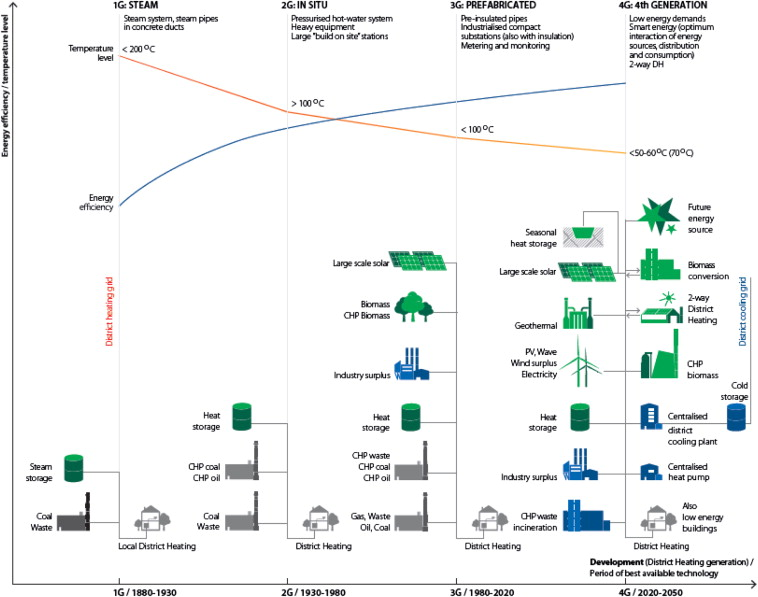
\includegraphics[width=1\textwidth]{4GDH.jpg}
\caption{The evolution of the district heating technology, from the 1st to the 4th generation. Source: \cite{lund4thGenerationDistrict2014}}
\label{fig:4GDH}
\end{figure}

District cooling (DC) networks had a similar development as DH networks, although to a smaller extent. 
% As seen in previous chapter, cooling demand will increase, especially for commercial applications. As for district heating in cold climates, in order to satisfy the future demand, several countries plan to develop the infrastructure for district cooling. For example the city of Dubai, for which air conditioning represents over 70 per cent of electricity consumption, aims to meet 40 per cent of its cooling needs through district
% cooling by 2030, using 50 per cent less electricity than standard air conditioning.\cite{unitednationsenvironmentprogrammeunepDistrictEnergyCities2015}

\subsection{Fifth generation district energy networks}\label{ss:5gden}
The 4th generation of DH technology, has already achieved remarkable success and has been widely applied, especially in Europe. However, the exergy losses of the system are still very high, due to the diversity of heat levels present in the system, limiting its efficiency. Moreover, the integration of DC, which, as it was mentioned beforehand is already important in cities and will become more and more important throughout the next years, needs the installation of a second and separate networks, which leads to high upfront costs. 

This has lead to the birth of a new technology that uses an even lower distribution temperature (10-25 \si{\celsius}) to provide heating and cooling. In fact, the transfer fluid acts as cold network for cooling purposes and supplies, at the same time, evaporator heat to decentralized heat pumps. This is what is known as the 5th generation DH networks, also known as District Energy Networks (DEN) or District Heating and Cooling (DHC). Besides the higher energy and exergy efficiency, which reduce the operating costs, this technology also reduces the upfront costs. Given the lower distribution temperature, in fact, the pipes require less insulation, as well as they can be placed in shallower depth in the ground.\\

This technology has appeared in Switzerland in 2007, and it's mostly known as \textit{anergy network}, or in german \textit{Anergienetz}. To the authors knowledge, there are seven such systems operating by the end of the year 2018\cite{energieschweizFallbeispieleThermischeNetze2018}. A summary of a selection of four of them is shown in Table \ref{tab:anergieCH_sum}, while more detailed information can be found in the Appendix \ref{as:anergy_suisse}.\\

\begin{table}[h]
\centering
\caption{District energy systems in Switzerland}\vspace{2mm} 
\label{tab:anergieCH_sum} 
\begin{tabular}{llllllll}
\toprule
                                                                                      & \textbf{\begin{tabular}[c]{@{}l@{}}
                                                                                      	Anergienetz \\
                                                                                      	    ETH     \\
                                                                                      	Hönggerberg
                                                                                      \end{tabular}} & \textbf{\begin{tabular}[c]{@{}l@{}}Suurstoffi-\\ Areal\end{tabular}}                             & \textbf{\begin{tabular}[c]{@{}l@{}}Anergienetz \\ Friesenberg (FGZ)\end{tabular}} & \textbf{\begin{tabular}[c]{@{}l@{}}Genève-Lac-\\ Nations (GLN)\end{tabular}} \\
\midrule
\textbf{Location}                                                                     & Zürich                                                                             & Rotkreuz                                                                                         & Zürich                                                                            & Genève                                                                       \\
\textbf{Year of construction}                                                         & 2012 - 2026                                                                        & 2010 - 2020                                                                                      & 2011-2050                                                                         & 2008 - 2016                                                                  \\
\textbf{ERA [m2]}                                                                     & 475'000                                                                            & 172'421                                                                                          & 185'000                                                                           & 840'000                                                                      \\
\textbf{\begin{tabular}[c]{@{}l@{}}Inst. Heating\\ capacity [kW]\end{tabular}}        & 8'000                                                                              & 6'732                                                                                            & 3'930                                                                             & 4'300                                                                        \\
\textbf{\begin{tabular}[c]{@{}l@{}}Heating demand \\ '[MWh/a]'\end{tabular}}          & 28'450                                                                             & 10'619                                                                                           & 35'000                                                                            & 5’000                                                                        \\
\textbf{\begin{tabular}[c]{@{}l@{}}Inst. Cooling\\ capacity [kW]\end{tabular}}        & 6'000                                                                              & 2'327                                                                                            & 3'500                                                                             & 16'200                                                                       \\
\textbf{\begin{tabular}[c]{@{}l@{}}Cooling demand \\ '[MWh/a]'\end{tabular}}          & 26'200                                                                             & 2'364                                                                                            & 80'000                                                                            & 20'000                                                                       \\
\textbf{Distribution fluid}        & water                                                                              & water                                                                                            & water                                                                            & water                                                                       \\
\textbf{Heat source}                                                                  & \begin{tabular}[c]{@{}l@{}}Laboratories\\ waste heat \\ +HP\end{tabular}           & \begin{tabular}[c]{@{}l@{}}Waste heat \\ buildings \\ + PVT (solar th.) \\ +HP\end{tabular}      & \begin{tabular}[c]{@{}l@{}}Waste heat\\ data center+HP\end{tabular}               & Lake water +HP                                                               \\
\textbf{Heat storage}                                                                 & \begin{tabular}[c]{@{}l@{}}Geothermal well \\ field\\ (431 at 200m)\end{tabular}   & \begin{tabular}[c]{@{}l@{}}Geothermal well\\ field \\ (215 at 150 m,\\ 180 at 280m)\end{tabular} & \begin{tabular}[c]{@{}l@{}}Geothermal well\\ field\\ (332 at 250m)\end{tabular}   & None                                                                         \\
\textbf{T of heating pipe}                                                                & 24 \si{\celsius} - 8 \si{\celsius}                                                                       & 25 \si{\celsius} - 8 \si{\celsius}                                                                                     & 28 \si{\celsius} - 8 \si{\celsius}                                                                      & 17 \si{\celsius} - 5 \si{\celsius}                                                                 \\
\textbf{T of cooling pipe}                                                                & 4 \si{\celsius} - 20 \si{\celsius}                                                                       & 4 \si{\celsius} - 17 \si{\celsius}                                                                                     & 4 \si{\celsius} -24 \si{\celsius}                                                                       & 5 \si{\celsius} - 12 \si{\celsius}                                                                 \\
\textbf{\begin{tabular}[c]{@{}l@{}}Tot. investments\\ '[Mio.CHF]'\end{tabular}}       & 37                                                                                 & n/a                                                                                              & 42.5                                                                              & 33                                                                           \\
\textbf{\begin{tabular}[c]{@{}l@{}}
	Tot. COP of heating \\
	  (incl. Pumps…)
\end{tabular}} & 5.8                                                                                & 2.7                                                                                              & 4.1                                                                               & 6.5                                                                            \\
\bottomrule
\end{tabular}
\end{table}


All the anergy networks presented in Table \ref{tab:anergieCH_sum} still base on water as a working fluid. Therefore, they work on sensible heat, which means that a heat exchange is bound to a variation in the fluids temperature. The challenge of these systems is given by the flow rate that is necessary to limit the temperature difference between the inlet and the return temperature of the network. Thus, it could be very interesting to use refrigerants, instead of water, that enable to work with latent heat instead, which means collecting and distributing heat through the condensation, or the evaporation, of the refrigerant. This poses some additional technological challenges, but has also very clear advantages, as it will be shown in the next chapters.\\

\begin{figure}[h!]
	\centering
	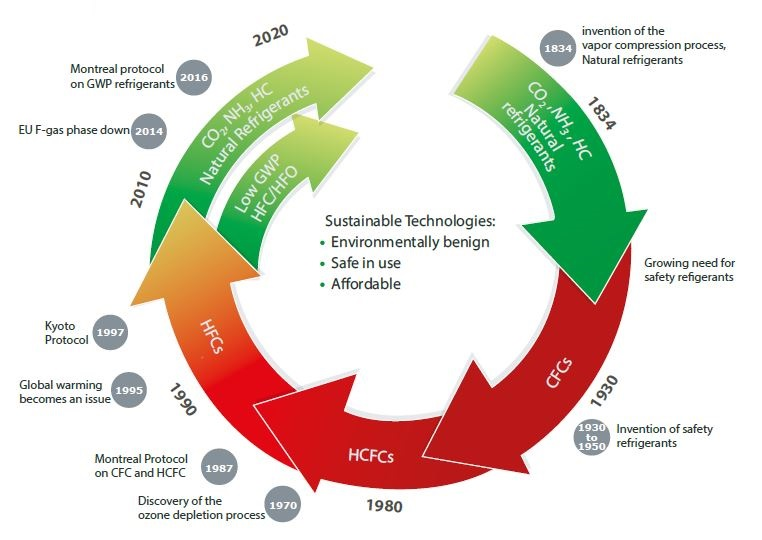
\includegraphics[width=0.6\textwidth]{refrigerants.JPG}
	\caption{The historical cycle of refrigerants Source: \cite{danfossRefrigerantOptionsNow2017}}
	\label{fig:refrigerants}
\end{figure}

The choice of the refrigerant strongly depends on the application. In function of the operating conditions, three main criteria are evaluated: affordability, safety and environmental impact.
A summary of the history of refrigerants is shown in Figure \ref{fig:refrigerants}.
The Montreal protocol, signed in 1987, designed the phase out of HCFC and CFCs, in order to prevent ozone layer depletion. This boosted the use of HFCs, as a replacement. However, not far later, people realized that despite being less damaging to the ozone layer, they were powerful greenhouse gases. Since 2013, a federal ordinance also strongly restricts the use of these last ones in Switzerland\cite{hydrocarbons21.comSwitzerlandIntroduceHFC}. Also Europe has planned the phase-out of HFC in 2014\cite{europeancommissionforclimateactionEULegislationControl2016}. This means that today the choice of refrigerants is essentially limited to natural refrigerants - as for example CO2 (R744), ammonia (R717) or propane (R290) - and the new environmentally friendly HFOs - as for example the fluorinated propane isomer R1234yf.\\

The choice of CO2 as a refrigerant relies, besides its thermodynamic properties, on the following arguments\cite{cavalliniPROPERTIESCO2REFRIGERANT}:
\begin{itemize}
	\item it is very abundant in the environment and is also waste of a multitude of industrial processes
	\item it is harmless to the biosphere
	\item it is non-flammable and non-toxic
	\item it is an inert gas
\end{itemize}

In fact, according to Danfoss\cite{danfossRefrigerantOptionsNow2017}, CO2 will dominate industrial refrigeration, together with ammonia. Already today, this technology is widely used. For instance Migros, Switzerland's largest retail company, opened its first supermarket to use CO2, in a low-temperature subcritical system, in 2002. By today, 411 of the 700 supermarkets in Migros’s portfolio are equipped with transcritical CO2 systems\cite{williamsMigrosDNA2018}.


\subsection{CO2 DEN}

%Generally, however, refrigerant based DEN are still at a prototype stage.

\subsubsection{The technology}
Weber and Favrat \cite{weberConventionalAdvancedCO22010a} compared the performance of a DEN using subcritical CO2, the HFO R1234yf and water. They were able to show that the CO2 network performs best, and has the biggest potential for DEN systems\cite{henchozPotentialRefrigerantBased}. 
As explained above, a refrigerant based DEN technology allows to store and transfer heat through the latent heat of vaporization of the refrigerant. The operating pressure is chosen in order to obtain the desired temperature in the system. That temperature is selected to be as high as possible to represent a good heat source for the decentralized heating heat pumps - resulting in good COP values -, while still allowing free cooling - avoiding the installation of compression chillers, and thus drastically reduce electricity consumption for space cooling. 

The network consists of one saturated liquid pipe and of one saturated vapor pipe, both in a saturated temperature range from 12 to 18 \si{\celsius}\cite{suciuEnergyIntegrationCO22018}.
The working principle is shown in Figure \ref{fig:CO2schema}. Heating users can extract heat from the network through condensation of the refrigerant, taken from the vapour pipe. Respectively, cooling users take refrigerant from the liquid pipe and evacuate heat by evaporating it. The heat exchanges between the network and the users occur through condenser-evaporators heat exchangers, which keep the different refrigerant loops isolated\cite{henchozPotentialRefrigerantBased}. The synergy between simultaneous heating and cooling users allows the recovery of waste heat. Most of the time, the required heating and cooling capacity will not be equal, which means that there is the need for a centralized balancing power. Indeed, a central plant is responsible to balance the overall network, by exchanging heat with the environment. For instance, a sole/water or a water/water heat pump can be used for this purpose.\\

%A comparison of the energy performance of two refrigerant based networks, CO2 and HFO R1234yf, and one cold water
%(anergy) network can be found in Ref.:
%S. Henchoz, P. Chatelan, F. Maréchal, and D. Favrat, “Key energy and technological
%aspects of three innovative concepts of district energy networks,” in Proceedings Of
%the 28th International Conference On Efficiency, Cost, Optimization

\begin{figure}[h!]
\centering
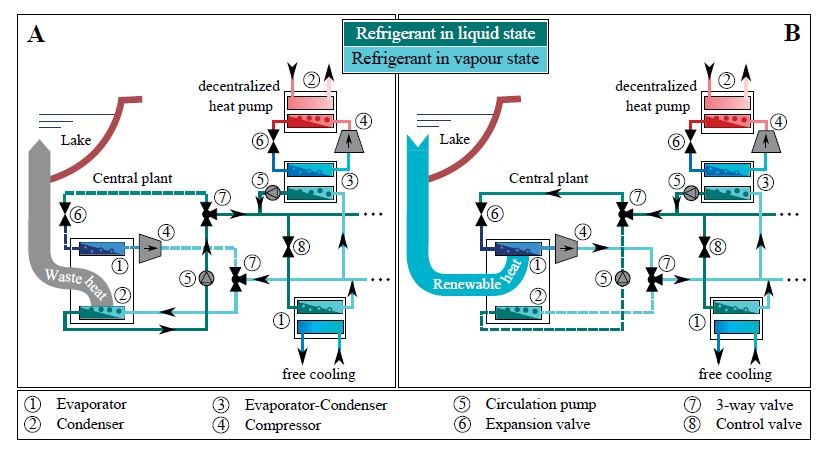
\includegraphics[width=1\textwidth]{CO2schema.JPG}
\caption{Schematics of a refrigerant based district energy network. Part A represents its net cooling operation, and part B its net heating operation. Source: \cite{henchozPotentialRefrigerantBased}}
\label{fig:CO2schema}
\end{figure}

One of the big advantages of this technology, with respect to water based DEN, is the pipes sizing. In fact, given the fact that it works on pressure maintenance instead of a fluid flow, no return pipe is necessary, which results in a slightly shorter total length of installed pipes. Moreover, due to the higher energy density of latent heat, the pipes diameter is drastically reduced. Henchoz et al. \cite{henchozPotentialRefrigerantBased} compared three different working fluid on the same study case, showing that, while CO2 needs pipes of only 280/330mm (liquid/vapor), R123yf would need 270/700mm and water 625/625mm. Given the low operating temperatures, there are much lower requirements for pipes insulation. While water pipes need to be buried deep enough to prevent damage due to water freezing, in case part of the network had to be stopped during winter, CO2 does not freeze and thus does not require a minimum freeze-safe depth. Henchoz et al. have even imagined installing the pipes inside a sidewalk module, which would drastically simplify maintenance and inspection. Given the smaller diameter, it would also be possible to retrofit an old, high temperature district heating network, by placing the CO2 pipes inside the old water pipes. All the above mentioned advantages of using CO2, result in lower upfront costs. \\
%Another advantage is the possibility of up-scaling a network. Indeed, to upscale a water based anergy network would require 
\todo{CO2den: necessary to talk about the advantage of expanding network with additional compressor easier than for water??}

The main drawback of this technology is the high operating pressure, which situates at about 50 bars, and the safety concerns that could derive from the large amount of CO2 that could escape in case of a major leakage. Nevertheless, as described in \ref{ss:5gden}, CO2 refrigeration networks are already widely used in supermakets, and the technology is considered as safe. \\
\todo{CO2den: need more drawbacks? or write more about it?}
%\textit{Safety issues analyzed \cite{girardinSafetyIssuesCO2based2016}.\\}
%\textit{A cold water network is the second best option, although more expensive initially and thus less profitable, it has several advantages in terms of safety and availability of components.}

\subsubsection{Performance}
Henchoz et al.\cite{henchozPotentialRefrigerantBased} performed an analysis of the potential application of a CO2 based DEN in a district in the city of Geneva. A map of the district, called "Rues basses", is shown in Figure \ref{fig:henchoz_gva}.

\begin{figure}[!htb]
	\centering
	\begin{minipage}{.45\textwidth}
		\centering
		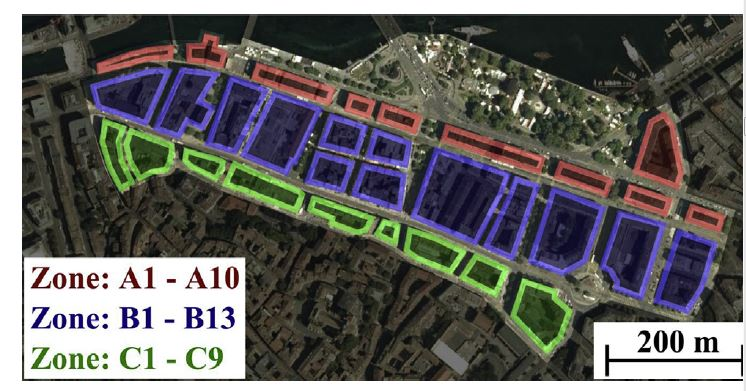
\includegraphics[width=\textwidth,height=0.2\textheight]{henchoz_gva.JPG}
		\caption{Representation of the the studied area and of its subdivision into 32 zones. Source: \cite{henchozPotentialRefrigerantBased}}
		\label{fig:henchoz_gva}
	\end{minipage}%
\hspace{1cm}
	\begin{minipage}{0.45\textwidth}
		\centering
		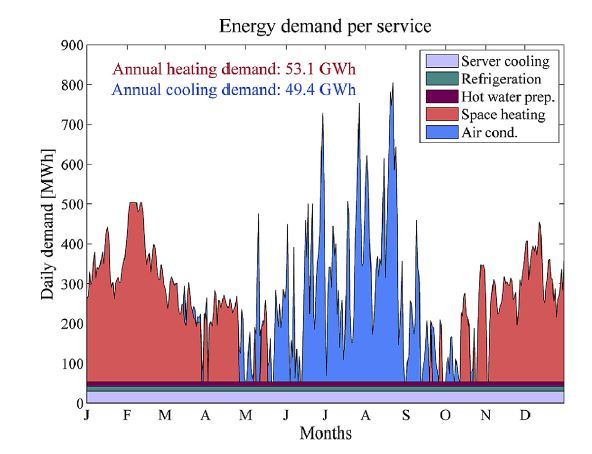
\includegraphics[width=\textwidth,height=0.2\textheight]{henchoz_energydemand.JPG}
		\caption{Energy demand for the area studied over the year 2012. Source: \cite{henchozPotentialRefrigerantBased}}
		\label{fig:henchoz_energydemand}
	\end{minipage}
\end{figure}


%\begin{figure}[h!]
%\centering
%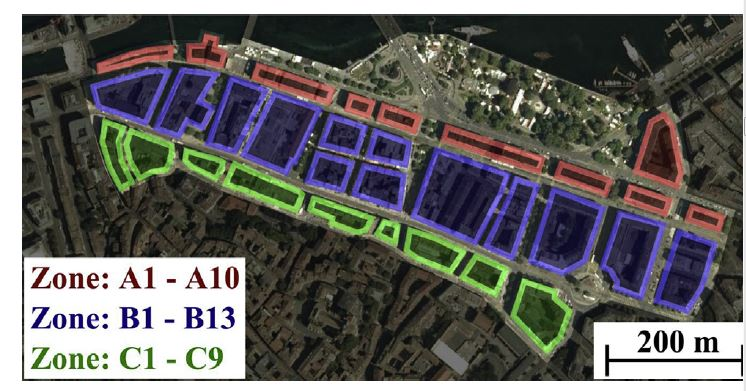
\includegraphics[width=0.5\textwidth]{henchoz_gva.JPG}
%\caption{Representation of the the studied area and of its subdivision into 32 zones. Source: \cite{henchozPotentialRefrigerantBased}}
%\label{fig:henchoz_gva}
%\end{figure}

Table \ref{tab:henchoz_area} shows the distribution of building affectations - which is important to determine the energy consumption - in the studied area. The total ERA is $687'800 m^{2}$.\\

\begin{table}[h!]
\centering
\caption{Distribution of the energy reference area for the different zones and building affectations}\vspace{2mm}
\label{tab:henchoz_area} 
\begin{tabular}{llll}
	\toprule
	Zones          & Commercial [$m^{2}$ ERA] & Offices  [$m^{2}$ ERA] & Residential  [$m^{2}$ ERA] \\ \midrule
	A1 - A10       & 20'700                   & 89'200                 & 17'700                     \\
	B1 - B13       & 97'000                   & 260'700                & 61'600                     \\
	C1 - C9        & 40'400                   & 62'600                 & 48'100                     \\ \midrule
	Relative share & 23\%                     & 60\%                   & 17\%                       \\ \bottomrule
\end{tabular}
\end{table}

The energy demand of heating ($53.1 GWh/yr$) and cooling ($49.4 GWh/yr$) in the studied area is shown in Figure \ref{fig:henchoz_energydemand}. Throughout the year, the district presents nearly the same heating demand as for cooling, but they happen in different seasons. 

%\begin{figure}[h!]
%\centering
%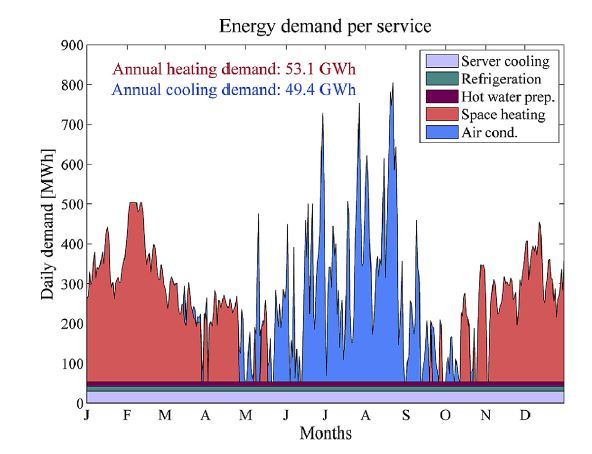
\includegraphics[width=0.75\textwidth]{henchoz_energydemand.JPG}
%\caption{Energy demand for the area studied over the year 2012. Source: \cite{henchozPotentialRefrigerantBased}}
%\label{fig:henchoz_energydemand}
%\end{figure}

The proposed CO2 based DEN is balanced by a central plant - a heat pump - that exchanges heat with the nearby lake. In order to benchmark the results, this technology has been compared to a traditional heating and cooling system, based on oil boilers and cooled compression chillers.

The results are remarkable. In fact, the CO2 based DEN shows a final energy consumption of 10,968 MWh of electricity, which corresponds to a reduction of 84.4 \%, with respect to the reference scenario. Its exergy efficiency situates between 40-45\%.

\todo{CO2gva: Talk about financial numbers comparison? Otherwise delete fig \ref{fig:henchoz_costs}}

\begin{figure}[h!]
\centering
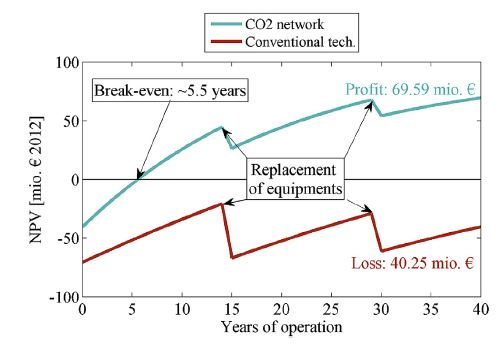
\includegraphics[width=0.5\textwidth]{henchoz_costs.JPG}
\caption{Evolution of the net present value over the lifetime of the two energy conversion technologies. Source: \cite{henchozPotentialRefrigerantBased}}
\label{fig:henchoz_costs}
\end{figure}


\subsubsection{Integration in smart energy system}
The integration of high shares of renewable energies represents an important challenge. In fact, it requires a lot of slack to handle the volatile nature of renewable energy sources like wind or sun. On one side, this slack will be mainly given through a smart control of the electricity grid on multiple levels. It starts from the demand side management (DSM) inside households, through optimization at district level, up to a national and international control. These decentralized grids, or grid controls, are called \textit{smart grids}. \\

With the vast success of heat pumps throughout the last decade, the control of electricity grids is more and more interconnected with the production of heat. This further complexifies the system by adding a level of constraints, but it also opens new levels of control. Indeed, if well designed, a DEN offers an additional level of slack that can be used in combination with the smart grid, multiplying control power. The CO2 DEN offers several possibilities to shift the loads, relieving the grid. \\

On one hand, it simplifies the deployment of a smart control of the heat pumps, which can strongly contribute in the DSM. The decentralized heat pumps can make use of a buildings thermal inertia to adapt electricity use to energy availability. CO2 vapor and liquid storage can act as a buffer, enabling load-shifting also for the central plant of the DEN. Sizing of these storage capacities will determine the possible time-span that the shift can achieve. Given the low distribution temperature, this approach also facilitates the storing of heat, as for example in a geothermal field.

On the other hand, the use of CO2 as a refrigerant for the network could improve the integration of a power to gas (PtG) system. Indeed, one big challenge in the future, especially in higher latitudes, where seasonal variation are consistent, is to ensure energy supply during winter season, when, due to shorter and weaker solar irradiation, PV panels produce less. It is thus important to find a way to store the excess of renewable energy production during the summer, in order to use it in the winter.
One solution to do that is PtG, which defines the process of transforming electrical power to a gas, like methane, which is easy to store. To do so, electricity is used to produce hydrogen, which can be combined with CO2 to form Methane, in a process called methanization. Methane can be used during the winter to produce electricity and heat, in a combined heat and power plant (CHP), as for example a SOFC, a gas turbine, or a combination of them. For this reason, PtG is widely studied across Europe and many such plants have already been built.\\ 
Suciu et al. \cite{suciuEnergyIntegrationCO22018} studied the synergy between a CO2 based DEN, decentralized PV and such a PtG system. The CO2 network could be used to store the carbon dioxide, which is captured from CHPs or industrial processes during winter, needed for methanization. At the same time, the DEN can directly use and dispatch the heat produced from the CHPs. In their work, they analyzed the PV area, and thus the investment, required to achieve a completely autonomous energy system, for different European climatic zones. The results showed that decarbonized autonomous energy systems based on DENs and PtG tecnologies are possible, along with a very broad deployment of solar energy. It is also shown that the payback time of such a system is between 11 and 14 years, which makes it very attractive also from an economic point of view.

\subsection{Direct-expansion ground source heat pump}\label{ss:dx}
\todo{where to put this section?}

For heat pumps based systems, sourcing heat from the sole, instead of from the ambient air, is a very interesting solution at our latitudes, especially, as it has been seen, for integration of a 5th generation DEN, since it improves heating and cooling COPs, and, to a certain extent, it allows heat storage. In traditional Ground-Source Heat Pumps (GSHP), the heat pump and the ground are connected by means of a closed loop, using water, or a water solution. This system, called the secondary loop GSHP (SL-GSHP), is shown on the right side of Figure \ref{fig:gshp}. However, it has been proved \cite{kruseStatusDevelopmentResearch, guoTechnoeconomicComparisonDirect2012} that the system efficiency can be improved, by allowing to directly expand the refrigerant into the ground and thus let the ground act as a condenser/evaporator. Shown on the left side of Figure \ref{fig:gshp}, this system is called Direct Expansion GSHP (DX-GSHP). 

\begin{figure}[h!]
\centering
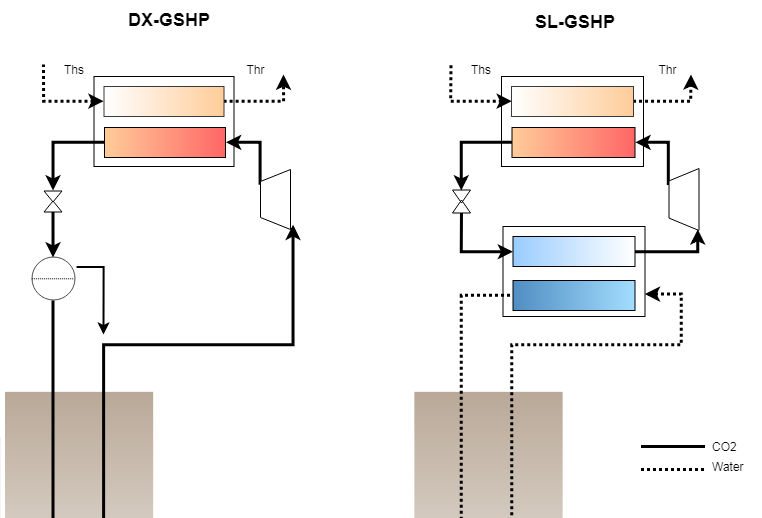
\includegraphics[width=1\textwidth]{GSHP.png}
\caption{A simplified schematics of the two GSHP technologies}
\label{fig:gshp}
\end{figure}

So far, this technology is not so widely spread, mostly because of a more demanding system design and, because of the risk of environmental pollution, when non-natural refrigerants are used. Indeed, literature about DX-GSHP is still scarce, especially for CO2 as a refrigerant. The are only few numerical CO2-DX-GSHP studies \cite{eslami-nejadModelingTwophaseCO2filled2014a,ghazizade-ahsaeeEnergyExergyInvestigation2018,austinParametricStudyPerformance2011,eslami-nejadQuasitransientModelTranscritical2015}, which are not yet sufficient to obtain a scientific appreciation of the technology. Nevertheless several prototypes and experimental set-ups have been built and analyzed \cite{eslami-nejadDetailedTheoreticalCharacterization2018, badacheExperimentalStudyCarbon2018, guoTechnoeconomicComparisonDirect2012}, proving a higher efficiency of the DX, with respect to a SL.

On of the main reasons for this efficiency gain is the elimination of the temperature lift of the water loop, which is replaced by a constant temperature phase-change, as well as the elimination of the minimum approach temperature necessary to exchange heat between the SL and the heat pump. This results in a higher COP for the heat pumps. 
Moreover, CO2 presents a higher heat transfer coefficient, which again allows to either reduce the minimum approach temperature, or extract a higher power with respect to an equal exchange surface. The minimum approach temperature has to be determined in function of the thermal permeability of soil and is correlated to the length and total surface of the geothermal probes, as well as the refrigerant flow rate.

\missingfigure{graph Q(T) for DX-GSHP}
 

\subsection{optimization}

\subsubsection{MILP}
Mixed integer linear programming (MILP) is... \\
AMPL a programm, solver using Gurobi, GLPK...\\
Black box??.....\\
State variables $X_{state}$\\
Model $F_{X_{state}}$\\
Context specification $S_{X_{state}}$\\
Inequality constraints $G_{X_{state}}$\\
\todo{find cheatsheet of exam MOES to do that}


%\subsubsection{Genetic algorithms}
%Optimization can be done through empirical algorithms that respect a set of rules. However, it is also possible to explore a space of solutions by reproducing the idea of evolution.
%
%\begin{enumerate}
%\item Create the population
%\item Determine fitness
%\item Select the mating pool
%\item Breed
%\item Mutate
%\item Repeat
%\end{enumerate}
%
%https://blog.sicara.com/getting-started-genetic-algorithms-python-tutorial-81ffa1dd72f9
%https://towardsdatascience.com/evolution-of-a-salesman-a-complete-genetic-algorithm-tutorial-for-python-6fe5d2b3ca35


\subsection{Osmose}\label{ss:osmose}
IPESE developed in-house software for this
Lua language
Layers, ETs...
Equations (mass balances, resource balances, heat cascade...)
Creates mod files for ampl optimization
Postcompute to export


Energy conversion technology sizing.
\begin{align}
& f_{u,t} \leq f_{u} \forall \qquad \forall u \in U, \ \forall t \in T  \\
& f_{u}^{min} \cdot y_{u} \leq f_{u} \leq f_{u}^{max} \cdot y_{u} \qquad \forall u \in U\\
\end{align}

For \textit{process units}, only the houses, $y_{u} = f_{u}^{min} = f_{u}^{max} = 1$\\

Heat cascade
A set of equantions, called heat cascade, makes sure that heat is always transferred from a higher temperature to a lower one, also considering the respective minimum approach temperature for each stream.
\begin{align}
& \sum_{u}^{U} f_{u,t}  \cdot \dot{Q}_{u,t,k} + \dot{R}_{t,k+1} - \dot{R}_{t,k} = 0 \qquad \forall k \in K, \ \forall t \in T \\
& \dot{R}_{t,k} \geq 0 \qquad \forall k \in K, \ \forall t \in T  \\
& \dot{R}_{t,1} = \dot{R}_{t,k+1} = 0 \qquad \forall t \in T  \\
\end{align}
\todo{is third eq rtk+1 = 0 correct???}

Mass balances
The demand $\dot{m}_{r,u,t}^{+}$ and the supply $\dot{m}_{r,u,t}^{-}$ of resource $r \in R$ of each unit $u \in U$ is computed.
\begin{align}
& \dot{M}_{r,u,t}^{-} = \dot{m}_{r,u,t}^{-} \cdot f_{u,t} \qquad \forall r \in R, \ \forall u \in U, \ \forall t \in T \\
& \dot{M}_{r,u,t}^{+} = \dot{m}_{r,u,t}^{+} \cdot f_{u,t} \qquad \forall r \in R, \ \forall u \in U, \ \forall t \in T  \\
\end{align}
The balance of each resource has to be respected.
\begin{equation}
\sum_{u}^{U} \dot{M}_{r,u,t}^{-} = \dot{M}_{r,u,t}^{+} \qquad \forall r \in R, \ \forall t \in T
\end{equation}
Electricity is also balanced
\begin{equation}
\dot{El}_{houses}^{+} + \dot{El}_{heating}^{+} + \dot{El}_{cooling}^{+} + \dot{El}_{grid}^{+} = \dot{El}_{PV}^{-} + \dot{El}_{grid}^{-}
\end{equation}

Opitmization function

\begin{align}
& min \left( TotalCost \right)  = min \left(  CAPEX + OPEX \right) \\
& min \sum_{u}^{U} ... \\
\end{align}

\begin{align}
& min \left( Operating cost \right) \\
& min \sum_{u}^{U} \left[ \sum_{t = 1}^{T} \left( c_{u}^{op1} \cdot y_{u,t} + c_{u}^{op2} \cdot f_{u,t} + C_{el}^{-} \cdot \dot{El}_{grid,t}^{-} - C_{el}^{+} \cdot \dot{El}_{grid,t}^{+} \right) \cdot t_{t}^{op} \right] \\
\end{align}

where $c_{u}^{op1}$ and $c_{u}^{op1}$ are the respectively the fixed and the variable operating cost, and $C_{el}^{-}$ and $C_{el}^{+}$ are the buying and selling price of electricity.

ET energy technologies:

The needed parameters are:
\begin{itemize}
	\item cinv1: fixed part of the IC, given in $[CHF/year]$. This can be found in figure \ref{fig:lin};
	\item cinv2: variable part of the IC, given in $[CHF/year]$. This can be found in figure \ref{fig:lin};
	\item cop1: fixed part of the OC, which corresponds to maintenance and service costs. 
	\item cop2: variable part of the OC. This is calculated by the solver, also in $[CHF/h]$.
\end{itemize}

\section{Methodology}

\subsection{Energy demand / Typical days}
According to SIA standards

Threshold temperature for heating or cooling
\todo{add this paragraph}


The optimization of an energy system is commonly performed over the time span of one year, in order to account for the different seasons. However, this requires a very long computing time, given the high number of timesteps. Thus, it is used to group similar days, according to a set of parameters as for example temperature or irradiation, into so called typical days. The days can be clustered in different ways. It can be chosen to compute an average day for each month or some machine learning clustering algorithm - as for example K-means, DBSCAN or GMM - can be used to group the days into the desired number of clusters.
The resulting typical days correspond to a period $p$, with a number of times $t$, as explained in section \ref{ss:osmose}. In order to account for the data compression, a value called $occurrence$ indicates how many times a given typical day occurs, i.e. how many times a given period occurs.\\

Two additional days with the two opposite extreme temperature conditions are added to the typical days, in order for the model to account for them in the equipment sizing. To avoid a bias of the operation results, those days are set with an occurrence of zero.


\subsection{Geothermal wells}\label{ss:gtw}

The most important parameter in geothermal wells is the soil temperature, which is normally constant throughout the year. In fact, only the first 10 meters are influenced by the temperature of the air\cite{hanSensitivityAnalysisVertical2016}. Moreover, the temperature increases with depth. According to the SIA norm SIA384\cite{siaSIA384Sondes2010}, the mean temperature in a geothermal well can be calculated by:
\begin{equation}
T_{g, mean} = T_{g,sup} + \frac{L_{w} \cdot \nabla T_{g}}{2}
\end{equation}
where $T_{g,sup}$ is the ground temperature at the surface, $L_{w}$ is the length of the well and $ \nabla T_{g}$ is the temperature gradient of the soil.\\

As for other technologies, the energy demand of the circulating pumps is assumed to be negligible. 

\subsection{Investment cost function}\label{ss:ic}
To calculate the investment cost for a given technology, it is possible to interpolate data from available products on the market. However, it is also possible to evaluate a cost function, according to a standard procedure in industrial processes\cite{turtonrichardc.bailierichardwhitingwallace.AnalysisSynthesisDesign2003}.

First, it is necessary to calculate the cost of purchase of the unit, in function of its size, given by the sizing power, which can be the electrical power $E$, the delivered heat $Q$ or the area of a heat exchanger $A$.

\begin{equation}
C_{pex} = \frac{I_{t}}{I_{t,ref}} \cdot 10^ {(k_{1,ex} + k_{2,ex} \cdot \log(E/Q/A))}
\end{equation}

Through a factor called \emph{Bare Module Factor}, the accessory costs of transport, installation, connection are included in the calculation, obtaining the total investment costs

\begin{equation}
CBM_{ex} = C_{pex} \cdot FBM_{ex} \cdot e 
\end{equation}

where $e$ is the currency ration from USD to CHF. The annuities are calculated with the annualization factor ($af$) by the following formula, where $n$ is the assumed lifetime of the equipment in years, and $i$ the interest rate. 

\begin{align}
	& IC_{yearly,ex} = CBM_{ex} \cdot af 
	& af = \frac{i \cdot (1 + i)^n}{(1 + i)^n - 1}
\end{align}

This investment cost function is not a linear function. However, as described in Section \ref{ss:osmose}, to solve the MILP it is necessary to provide a set of linear parameters that approximate the function. These are found by linearizing the investment cost function around the reference value, defined in the range of application. This was done with help of a matlab code, using \textit{polyfit} and \textit{polyval} functions. Figure \ref{fig:lin} shows the linearized function with the according cost parameters.

\begin{figure}[htp]
	\centering
	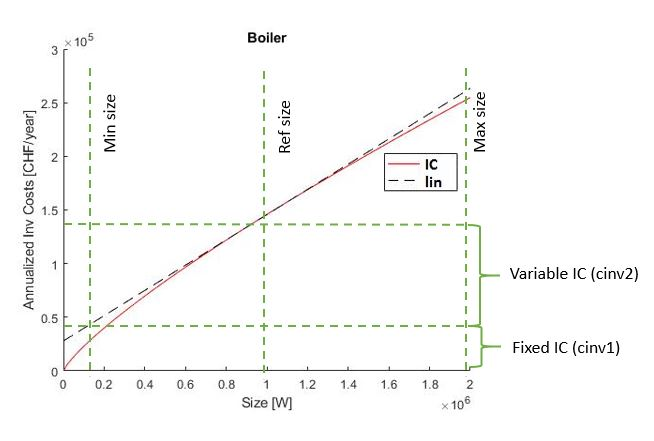
\includegraphics[scale=0.6]{Images/linearization_expl.jpg}
	\caption{Linearization of investment cost function}
	\label{fig:lin}
\end{figure}

\subsection{Minimum approach temperature}\label{ss:dtmin}
The critical sizing parameter for a heat exchange is the minimum approach temperature $\Delta T_{min}$, which corresponds to the smallest temperature difference in the heat exchanger between the hot and the cold stream, as shown in Figure \ref{fig:dtmin}. This value is strongly dependent from the heat exchanger area $A_{ex}$ and the heat transfer coefficients $h$ of the exchanging fluids. They are correlated in the following way: 

\begin{equation}\label{eq:HEX_area}
A_{ex} = \frac{Q_{ex}}{U \cdot LMTD}
\end{equation}
\begin{equation}\label{eq:LMTD}
LMTD= \frac{(T_{Hot,in } - T_{cold,out }) - (T_{Hot,out } - T_{cold,in }) }{ \log{ (\frac{T_{Hot,in } - T_{cold,out }}{T_{Hot,out } - T_{cold,in }} ) }}
\end{equation}
\begin{equation}
	T_{Hot,in } = T_{cold,out} + \Delta T_{min}
\end{equation}
where  $LMTD$ id the logarithmic mean temperature difference and T are the inlet and outlet temperatures of the hot and cold streams, as shown in Figure \ref{fig:dtmin}. The overall heat transfer coefficient is given by \cite{huExtremumSeekingControl2015}:
\begin{equation}\label{eq:alpha}
U= \frac{1}{ \frac{1}{h_{(hot)} } + \frac{\Delta x_{wall}}{k_{wall}} + \frac{1}{h_{(cold)}} }
\end{equation}
where $h_{(hot)}$ and $h_{(cold)}$ are the heat transfer coefficient of the hot and cold fluid, while $\Delta x_{wall}$ and $k_{wall}$ are respectively the thickness and the thermal conductivity of the heat exchanger plates.

\begin{figure}[htp]
	\centering
	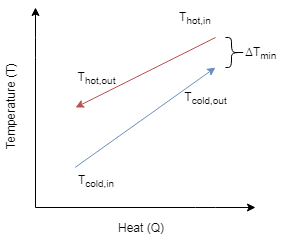
\includegraphics[scale=0.6]{Images/dtmin.png}
	\caption{Minimum approach temperature in a counter-flow heat exchanger.}
	\label{fig:dtmin}
\end{figure}

A bigger $A_{ex}$ allows a smaller $\Delta T_{min}$, which increases the investment costs but lowers the operating costs, and the other way around. Therefore, an optimum can be found for each specific application. 
The optimization is done by minimizing the total cost, which include the operating costs of a heat pump - whose COP decreases with $\Delta T_{min}$ -, and the investment costs of the heat exchanger and of the HP:
\begin{equation}
	\min_{\Delta T_{min}}\left\lbrace OC(\Delta T_{min}) + IC(\Delta T_{min}) \right\rbrace 
\end{equation}

\todo{dtmin finish rewriting this last part}
Heat transfer coefficients used are shown in Table \ref{tab:alphas}.
The values for for R134yf \cite{wangOverviewHeatTransfer2013}

while for CO2 from this paper\cite{ohFlowBoilingHeat2011}.
Validated also by comparison between the two\cite{mastrulloComparisonR744R134a2009}. 
\\

\begin{table}[h!]
\centering
\caption{Heat transfer coefficients found in literature}\vspace{2mm}
\label{tab:alphas} 
\begin{tabular}{llll}
	\toprule
	Fluid             & Water & R134yf & R744 \\ \midrule
	$h [W/(mK)]$ & 600   & 3000   & 7000 \\ \bottomrule
\end{tabular}
\end{table}


\subsection{Exergy}
\todo{Exergy: chapter not finished}
The exergy of a heat transfer is defined as the maximum amount of work that can be extracted from it, through reversible transformations that exchange with the environment. Thus the calculation of exergy losses is a very interesting indicator to analyze a given process or system, since it expresses the quality and the efficiency with which the system operates, with respect to the maximum possible. Therefore, these values are always lower than 100 \%. \\

The maximum work that can be extracted is derived from the first two thermodynamic principles, and is given by the following formula:
\begin{equation}
    \dot{E}^{-}_{max} = \sum_{i} \dot{Q_i}^{+} (1 - \frac{T_{a}}{T_i} ) + \sum_{r} \dot{M}_{r}^{+} (h_{r} - T_{a} s_{r})    
\end{equation}

In order to compute the exergy losses the general approach that can be used is the following:
\begin{equation}
    \dot{L} = \dot{E}^{-}_{max} - \sum_{j}\dot{E}^{-}_{j} \geq 0
\end{equation}

In our case
\begin{align}
    & \eta_{exergy} =  \frac{\dot{Q}_{cold,a} + \dot{Q}_{hot,r} + \dot{E}_{grid}^{-}}{\dot{Q}_{cold,r} + \dot{Q}_{hot,a} + \dot{E}_{grid}^{+}}  \\
    & \dot{L} = (1-\eta_{exergy})(\dot{Q}_{cold,r} + \dot{Q}_{hot,a} + \dot{E}_{grid}^{+})
\end{align}
where $\dot{Q}_{hot,a}$ and $\dot{Q}_{hot,r}$...?

\subsection{Energy technology models}\label{ss:et}
The models for the energy technologies are adapted from the source code written by Suciu Raluca.\todo{cite anything, or name is enough?}\\
thermodyn cycle from\cite{demierreModelingExperimentalInvestigation2014}\\
\todo{other names?}
\subsubsection{Heat pumps - basic (Carnot)}\label{sss:hp_carnot}
Heat pumps can be modeled in a simple way, using the principle of the Carnot cycle, with help of the following equations:
\begin{align}
    & \dot{E}_{compressor} = \frac{\dot{Q}_{cond}}{COP_{real}} = \frac{\dot{Q}_{evap}}{\eta_{COP} \cdot COP_{theoretical}} \\
    & COP_{theoretical, heating} =  \frac{T_{h}}{T_{h} – T_{c}}  
    & COP_{theoretical, cooling} =  \frac{T_{c}}{T_{h} – T_{c}} 
\end{align}
where $\dot{Q}_{cond}$ is the heat delivered and $\dot{Q}_{evap}$ the heat sourced by the heat pump. $\eta_{COP}$ is an experimentally defined efficiency to account for irreversibility of the cycle, i.e. to give the ratio between the theoretical and the real COP. The values used in this work are shown in Table \ref{tab:etaCOP}, calculated by Girardin et al.\cite{girardinEnerGisGeographicalInformation2010}, based on values obtained from c heat pump certification center\cite{NTBBuchsInstitut}. \\

\begin{table}[h!]
\centering
\caption{Theoretical efficiency factor for COP}\vspace{2mm}
\label{tab:etaCOP} 
\begin{tabular}{lll}
	\toprule
	Type         & Size          & $\eta_{COP}$ \\ \midrule
	Air/Water    & Decentralized & 0.34         \\
	CO2/Water    & Decentralized & 0.43         \\
	Ground/Water & Decentralized & 0.43         \\
	Ground/Water & Centralized   & 0.55         \\
	Water/Water  & Centralized   & 0.55        \\ \bottomrule
\end{tabular}
\end{table}


\subsubsection{Heat pumps - detailed (Thermodyn.)}\label{sss:hp_thermo}

\begin{figure}[htp]
	\centering
	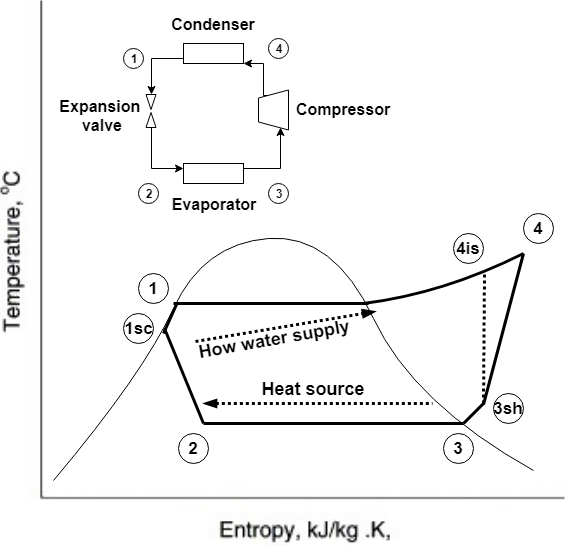
\includegraphics[width=0.5\textwidth]{HP_cylce_ref.png}
	\caption{Temperature–entropy diagram of a R134yf based heat pump system.}
	\label{fig:hp_ref}
\end{figure}

Given the comparison between new and efficient technologies, the differences of performance are relatively small and it might be necessary to provide a more accurate model of the heat pumps, that are able to correctly represent and calculate the operating cycles and conditions. This can be done by modeling the thermodynamic cycle, represented in Figure \ref{fig:hp_ref}:

\begin{description}
	\item [1 - 2]: Expansion to low pressure level
	\item [2 - 3]: Evaporation by cooling down the heat source
	\item [3 - 3sh]: Superheating in evaporator
	\item [3sh - 4]: Compression to high pressure level
	\item [4 - 1]: Condensation of refrigerant, delivering heat
\end{description}

The compressor is a crucial component for the design of a heat pump, since it has the largest share of impact on the energy efficiency. To calculate its efficiency, the model of Hu et al.\cite{huExtremumSeekingControl2015} has been used. The shaft power can be computed in function of the isentropic efficiency ($\eta_{is}$) by:
\begin{equation}
W_{shaft} = \frac{\dot{m}(h_{d,is}-h_{s})}{\eta_{is}} 
\end{equation}
where $h_{d,is}$ is the isentropic discharge enthalpy and $h_{d}$ is the suction enthalpy. The compressors input power is expressed in function of its mechanical efficiency ($\eta_{is}$) by:
\begin{equation}
E_{comp} = \frac{W_{shaft}}{\eta_{mech}}  
\end{equation}
The efficiency of the compressor is thus calculated as:
\begin{equation}
\eta_{comp} = \frac{\text{isentropic work of compression}}{\text{actual work of compression}} = \frac{\dot{m}(h_{d,is}-h_{s})}{E_{comp}} = \eta_{is}\eta_{mech} 
\end{equation}

The numerical values of those efficiencies are strongly dependent from the ratio between the pressure of discharge $P_{d}$ and the pressure of suction $P_{s}$ of the compressor.They can be computed inside the model with help of the relations obtained by Li et al.\cite{liPerformanceCharacteristicsR1234yf2014}:
\begin{align}
& \eta_{mech} = 0.85\\
& \eta_{is} = 0.874-0.0134\cdot(\frac{P_{d}}{P_{s}})\\
\end{align}
		
The expansion of the refrigerant in the expansion valve is assumed to be isenthalpic.\\ 

Thus, the procedure to evaluate the operating conditions of the heat pump is the following:
\begin{enumerate}
	\item calculate thermodynamic state in point (1) knowing the evaporation temperature $T_{evap}$ and assuming saturated liquid
	\item calculate thermodynamic state in (1sc) using same pressure as in (1), with $T = T_{evap} - \Delta T_{subcool}$
	\item calculate thermodynamic state in point (3) knowing the evaporation temperature $T_{cond}$ and assuming saturated vapor
	\item calculate thermodynamic state in (3sh) using same pressure as in (3), with $T = T_{cond} + \Delta T_{superheat}$
	\item calculate thermodynamic state in (2), assuming isenthalpic expansion of the valve, with $H_{2} = H_{1sc}$ and $P_{3}$
	\item calculate isentropic efficiency of compressor $\eta_{c,is}$, knowing the discharge pressure $P_{1}$ and the suction pressure $P_{3}$
	\item calculate thermodynamic state in (4is), assuming an isentropic compression with $S_{3sh}$ and $P_{1}$
	\item calculate thermodynamic state in (4), accounting for the isentropic efficiency of the compressor $\eta_{c,is}$, using $H_{4} = H_{3sh} + \frac{H_{4is} - H_{3sh}}{\eta_{c,is}}$, and $P_{1sc}$.
\end{enumerate}

In Osmose, these values are calculated with help of \textit{Coolprop}, which is an open-source database of fluid and humid air properties that allows to calculate operating conditions for a large number of fluids and refrigerants. Thanks to a \textit{lua wrapper}, which is a \textit{lua} module that provides an API to the external software, \textit{Coolprop} is called inside Osmose.

The electrical power of the heat pump and its COP, are then calculated by:
\begin{align}
	& E_{el} = \frac{m_{ref} \cdot (H_{4}-H_{3sh})}{\eta_{mech}}\\
	& Q_{cond} = m_{ref} \cdot (H_{4}-H_{1sc})\\
	& COP = \frac{Q_{cond}}{E_{el}}
\end{align}
where $m_{ref}$ is the massflow of refrigerant in the heat pump.


\subsubsection{Heat pump - supercritical CO2}\label{sss:hp_CO2}

\begin{figure}[htp]
	\centering
	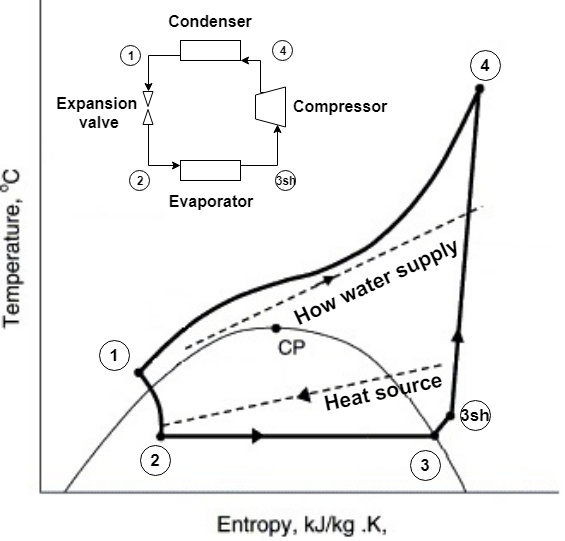
\includegraphics[width=0.5\textwidth]{HP_cylce_CO2.png}
	\caption{Temperature–entropy diagram of a trans-critical CO2 heat pump system for a domestic hot water production. Source: \cite{kimPerformanceTranscriticalCO22005}}
	\label{fig:hp_CO2}
\end{figure}

In traditional heat pumps, the heat delivery occurs through condensation of the refrigerant, which happens at a fixed temperature. This originates high exergy losses, especially in processes were a high temperature lift is needed in the gas cooler. Some refrigerants have the particular property of having a very low critical point. Among others, a very interesting one is CO2 - technically know as R744 -, which has a critical point at 74 bars and 31 \si{\celsius}\cite{cavalliniPROPERTIESCO2REFRIGERANT}. As explained in Section \ref{ss:5gden}, CO2 is also a very interesting choice for environmental and financial reasons.\\

The supercritical cycle is shown in Figure \ref{fig:hp_CO2}, represented on the temperature-entropy diagram. The different steps of the process are explained hereafter: 
\begin{description}
\item [1 - 2]: Expansion to low pressure level
\item [2 - 3]: Evaporation by cooling down the heat source
\item [3 - 3sh]: Superheating in evaporator
\item [3sh - 4]: Compression to transcritical pressure
\item [4 - 1]: Gas cooling in transcritical area, to heat water
\end{description}
Note that, as there is no phase change, the heat exchanger is called gas cooler, instead of condenser.\\

Even though the technological development is slowly closing the gap, CO2 compressors have lower isentropic efficiency and lower volumetric efficiency than subcritical ones\cite{sarkarSimulationTranscriticalCO22006}. This comes from the high irreversibility caused by the superheated vapor horn and the high throttling losses\cite{yangTheoreticalExperimentalInvestigation2016}. 
However, transcritical operation also allows heat to be exchanged on a varying temperature, and the heat pump can be designed to fit the heat demand stream, optimizing exergy efficiency. This is particularly interesting in exchanges that require high temperature lifts, as in the case of domestic hot water heaters. In fact, this can be seen in Figure \ref{fig:hp_CO2}, between point 2 and 3.  For instance, Stene et al. show that COP for a CO2 HP is lower if it is used in subcritial range - for Space Heating (SH) (35/30 \si{\celsius}) - than in supercritical range - Domestic Hot Water (DHW) (10/60 \si{\celsius}) -, despite the much higher temperature difference. They also show that the resulting COP for DHW application outperforms conventional HPs\cite{steneINTEGRATEDCO2HEAT2007}.\\

For the transcritical CO2 heat pump, the numerical values of the compressor efficiencies computed with help of the relations obtained by Wang et al \cite{wangExperimentalInvestigationAirsource2013}:
\begin{align}
	& \eta_{mech} = 0.64107+0.07487\cdot(\frac{P_{d}}{P_{s}})\\
	& \eta_{is} = 0.8014-0.04842\cdot(\frac{P_{d}}{P_{s}})\\
\end{align}

The procedure to evaluate the operating conditions of the heat pump is the following:
\begin{enumerate}
	\item calculate thermodynamic state in (1) with help of the temperature at the outlet of the condenser $T = T_{cond,out} = 15.5 \si{\celsius}$, optimized for this specific cycle by Henchoz et al.\cite{henchozPerformanceProfitabilityPerspectives2015}, and the pressure $P_{cond,out} = 84.9 bar$, optimized to satisfy the required inlet temperature of the condenser
	\item calculate thermodynamic state in point (3) knowing the evaporation temperature $T_{evap}$ and assuming saturated liquid
	\item calculate isentropic efficiency of compressor $\eta_{c,is}$, knowing the discharge pressure $P_{1}$ and the suction pressure $P_{3}$
	\item calculate thermodynamic state in (4is), assuming an isentropic compression with $S_{3sh}$ and $P_{1}$
	\item calculate thermodynamic state in (4), accounting for the isentropic efficiency of the compressor $\eta_{c,is}$, using $H_{4} = H_{3sh} + \frac{H_{4is} - H_{3sh}}{\eta_{c,is}}$, and $P_{cond,out}$.
	\item calculate thermodynamic state in (2), assuming isenthalpic expansion of the valve, with $H_{2} = H_{1}$ and $P_{3}$
\end{enumerate}

The equations to calculate electrical power of the heat pump and its COP, are the same as in Section \ref{sss:hp_thermo}.

\subsubsection{Cooling tower / Air cooler}\label{sss:cooling_tower}
A cooling tower is an equipment used to cool down a stream through the ambient air. This is used for example in air conditioning systems, to evacuate the heat into the environment. It consists of a set of fans that blow the air through a heat exchanger. These fans originate a parasitic power consumption that can be calculated with help of the following equation\cite{henchozPotentialRefrigerantBased}:
\begin{equation}
\dot{E_{fans}} = \frac{0.605 \cdot \dot{Q}_{cond}}{( \Delta T_{air} + \Delta T_{min}^{ref/air})^{0.9937}}
\end{equation}
Where $\dot{Q}_{cond}$ is the heat to be dissipated in the environment by the condenser. 


\subsubsection{Geo-cooling}
Geo-cooling is the use of fresh temperatures of the ground for space cooling. This happens by simply circulating a fluid between the buildings, where the heat is extracted, and the geothermal wells, where heat is released into the ground. In practice, this happens by bypassing the heat pumps and making the water of the secondary loop (geothermal loop) directly exchange with the heating water loop. Investment costs are, thus, limited to an additional heat exchanger. As for the other units, the energy needed for circulation pumps is assumed to be negligible. 


\subsubsection{PV}
The efficiency of the PV panels $\eta_{PV}$ is given by the following equation:
\begin{equation}
	\eta_{PV} = \eta_{ref} - \eta_{var} (T_{panel}-T_{ref})
\end{equation}
where $\eta_{ref}$ and $\eta_{var}$ are respectively the fixed efficiency and the temperature dependent efficiency. The temperature of the panel $T_{panel}$ is calculated by means of:
\begin{equation}
	T_{panel} = \frac{U_{glass}\cdot T_{amb} + GI \cdot f_{glass}-\eta_{ref} - \eta_{var} \cdot T_{ref}}{U_{glass}-\eta_{var} \cdot GI}
\end{equation}
where $U_{glass}$ is the thermal transmittance of the front glass, $f_{glass}$ is the light transmittance of the front glass and GI is the global irradiation.
Thus, the produced energy is given by:
\begin{equation}
	E = GI \cdot A_{PV} \cdot  \eta_{PV}
\end{equation}
The area of installed PV $A_{PV}$ is limited by the maximum available roof area multiplied by the area factor $f_{area}$, which for flat roofs is assumed to be $\frac{1}{4}$:
\begin{equation}
	A_{PV} = A_{roof} \cdot f_{area}
\end{equation}


\subsubsection{Network}\label{sss:net}
The length is calculated, according to a simplified method\cite{girardinEnerGisGeographicalInformation2010}, with the following equations:
\begin{equation}
L = 2(n_{b}-1)K\sqrt{\frac{S}{n_{b}}}
\end{equation}
with $S$ being the land area, $n_{b}$ the number of buildings. The constant $K$ is chosen at 0.5.
And diameter of the pipes:
\begin{equation}
d = \sqrt{\frac{4\cdot \dot{m}}{\pi v_{s} \rho}}
\end{equation}
assuming a sizing velocity $v_{s}$ of 3 m/s.
The investment costs are calculated accordingly:
\begin{equation}
C = \sum_{k=1}^{n_{b}} \frac{L}{n_{b}} (c_{1} d \sqrt{n_{b}+1-k} + c_{2})
\end{equation}
where $c_{1} =5670 $ and $c_{2} = 613 $.\\

Operating temperature is assumed to be 13/15 \si{\celsius}.
\todo{how has this temperature been chosen? is there a paper? see henchoz with other T}
Henchoz\cite{henchozPotentialRefrigerantBased} has 10-12.5 for summer and 22.5 for winter!!! 

The pressure losses, and thus the energy needed for the maintaining of the pressure, are assumed to be negligible.


\section{Application}

\subsection{Case-study Eglantine}\label{ss:Eglantine}
In the framework of the collaboration between Romande Energie and IPESE, a case study shall bring a concrete numerical case study into the discussion. For this, Romande Energie has chosen a real life example of a district in the city of Morges. This district is in the planning phase, and Romande Energie had worked on it, in order to participate in the call for tender. This case study shall be fertile ground to discuss the CO2 DEN technology and it's role in the future energy systems in Switzerland and, more particularly, in the future plans of Romande Energie.

\subsubsection{Context}

\begin{figure}[htp]
\centering
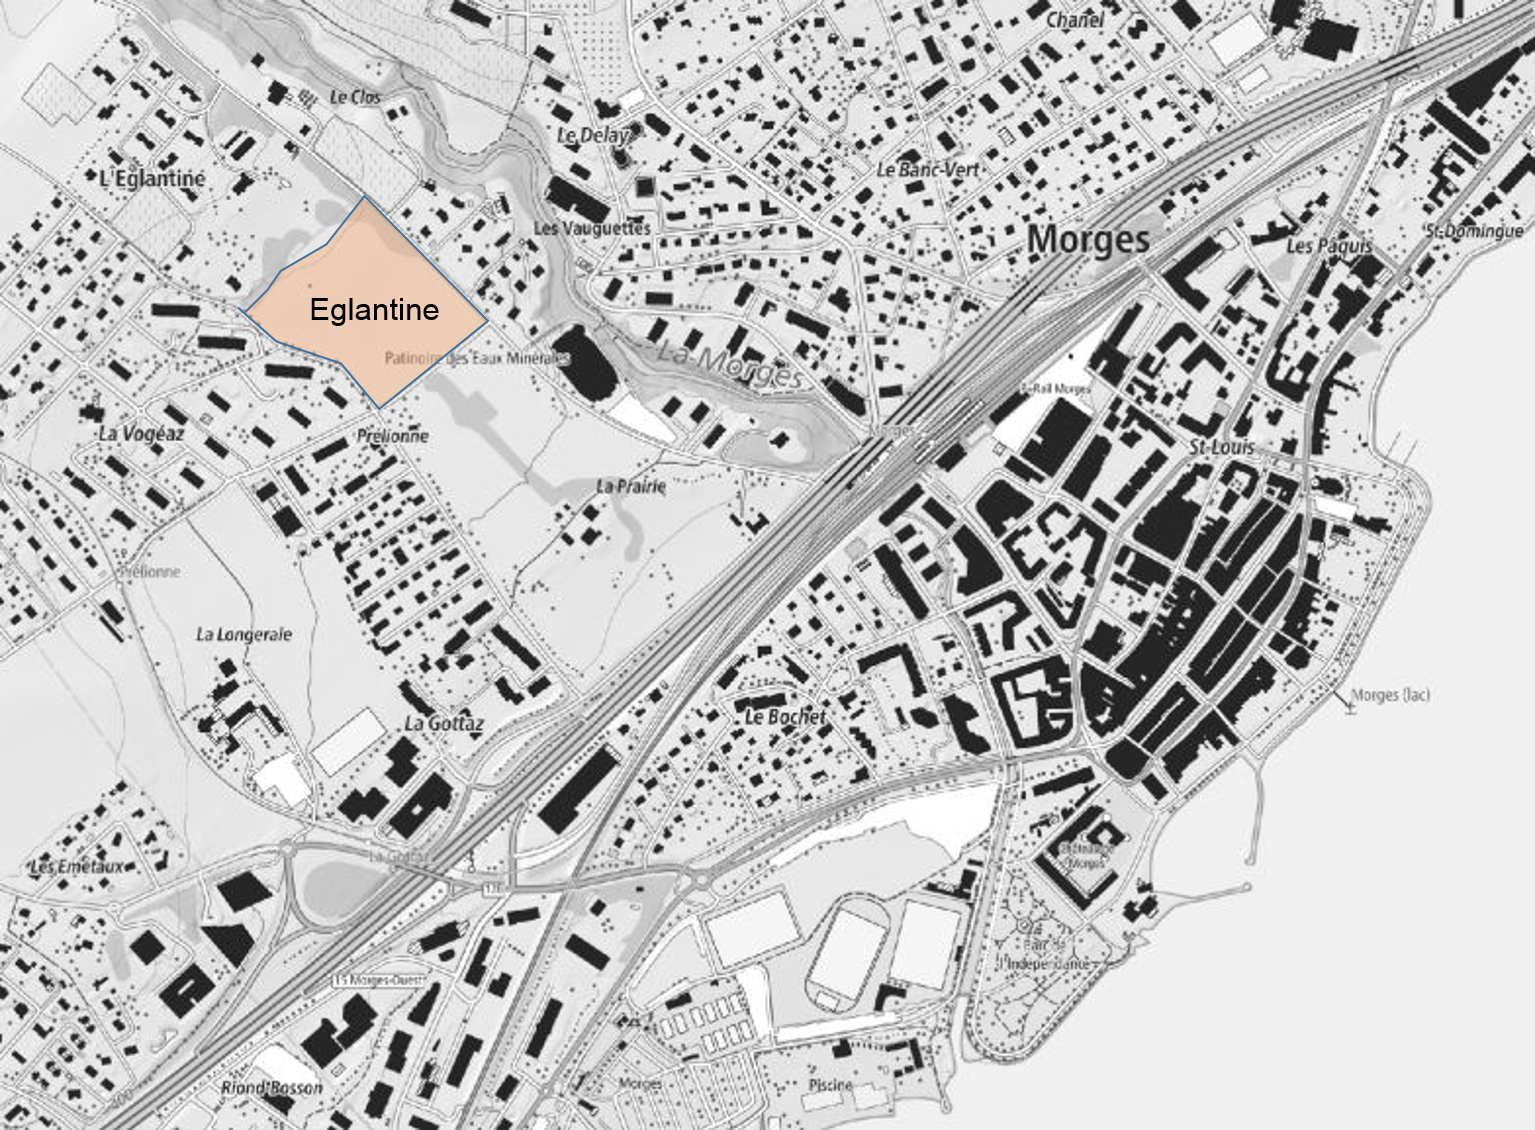
\includegraphics[width=1\textwidth]{morges.png}
\caption{Localization of the terrain, at the town scale. Source: www.geo.vd.ch}
\label{fig:morges}
\end{figure}

The “Eglantine” is a terrain in the western part of the city of Morges, as shown in Figure \ref{fig:morges}. It is located in proximity of the key urban facilities, as well as it is close to the countryside. This terrain, which was partly used for agriculture, and partly covered by rich vegetation, belongs to the municipality, who is planning to use it for the urban expansion. At the municipality, they had the vision of building a new district, which would be planned to be exemplary in the sustainable development. After many years of revising and fine-tuning the land-use plan and its vision for the future, in the beginning of 2016, the commune launched a call for tender for the planning of the different aspects of the district. The call for tender regarding the energy system was opened by Losinger Marazzi the 1st December 2017, with a due date the 31 January 2018. The contract with the winner, unknown to the author, has been signed in the end of March 2018. \\

The call for tender requires the development of a complete energy system, including thermal and electrical energy. Estimated data about the buildings is provided, as seen in Table \ref{tab:ppa_summary}. Those are based on the following assumptions:
\begin{itemize}
    \item All buildings are certificated Minergie 2017
    \item Space heating and hot water energy demand follow the SIA 380/1 and SIA 2031 norms
    \item Air ventilation is defined according to Minergie 2017 principles.
    \item Installed power values are calculated according to SIA 2024 norm
\end{itemize}

\subsubsection{Buildings}
The district, which will host around 1'500 people, is composed of thirteen buildings, as shown in Figure \ref{fig:ppa_buildings}, which account for a total energy reference area (ERA) of around $47'000 m^{2}$. The details are shown in Table \ref{tab:ppa_summary}. According to the Minergie standard, the district will require about $1.40 MWh/yr$ for SH and $0.95 MWh/yr$ for DHW.\\

\begin{table}[h!]
\centering
\caption{Estimated energy demand in call for tender}\vspace{2mm}
\label{tab:ppa_summary} 
\begin{tabular}{lrrrrr}
\toprule
\textbf{Building} & \begin{tabular}[c]{@{}l@{}}\textbf{Energy Ref.} \\ \textbf{Area (ERA)}\end{tabular} & \textbf{Inhabitants} & \begin{tabular}[c]{@{}l@{}}\textbf{Space Heating} \\ \textbf{(SH)}\end{tabular}                                             & \begin{tabular}[c]{@{}l@{}}\textbf{Hot Water} \\ \textbf{(DHW)}\end{tabular} & \textbf{TOTAL}     \\
         &                                                                        &             & \begin{tabular}[c]{@{}l@{}}MIINERGIE\\ simple flux\end{tabular} & SIA 380/1       &           \\
         & [m2]                                                                   &             & [kWh/yr]                                                        & [kWh/yr]        & [kWh/yr]  \\
         \midrule
1        & 8'200                                                                  & 273         & 245'180                                                         & 170'833         & 416'013   \\
2        & 2'615                                                                  & 76          & 82'308                                                          & 50'104          & 132'412   \\
3        & 2'415                                                                  & 70          & 76'328                                                          & 45'938          & 122'266   \\
4        & 2'780                                                                  & 92          & 83'122                                                          & 57'917          & 141'039   \\
5        & 3'700                                                                  & 116         & 113'246                                                         & 74'306          & 187'552   \\
6        & 1'500                                                                  & 50          & 44'850                                                          & 31'250          & 76'100    \\
7        & 2'870                                                                  & 83          & 90'652                                                          & 54'653          & 145'305   \\
8        & 2'500                                                                  & 83          & 74'750                                                          & 52'083          & 126'833   \\
9        & 4'225                                                                  & 140         & 126'328                                                         & 88'021          & 214'349   \\
10       & 4'455                                                                  & 148         & 133'205                                                         & 92'813          & 226'018   \\
11       & 4'190                                                                  & 139         & 125'281                                                         & 87'292          & 212'573   \\
12       & 2'300                                                                  & 76          & 68'770                                                          & 47'917          & 116'687   \\
13       & 2'300                                                                  & 76          & 68'770                                                          & 47'917          & 116'687   \\
14       & 2'300                                                                  & 76          & 68'770                                                          & 47'917          & 116'687   \\
\midrule
\textbf{TOT}      & \textbf{46'350}                              & \textbf{1'498}       & \textbf{1'401'559}      & \textbf{948'958}         & \textbf{2'350'521} \\
\bottomrule
\end{tabular}
\end{table}

The call for tender includes also information about the end use of the buildings, which is shown in Table \ref{tab:ppa_buildinguse}. It can be seen that the buildings include, beside the residential use (multidwelling), also a small share of retail and restaurant services use, which are associated with different energy needs. Moreover, there is even a small indoor swimming pool, located in building one. 

\begin{table}[h!]
\centering
\caption{Estimated use of buildings in call for tender}\vspace{2mm}
\label{tab:ppa_buildinguse}
\begin{tabular}{lllll}
\toprule
\textbf{Building} & \textbf{Multidwelling} & \textbf{Retail} & \textbf{Restaurant services} & \textbf{Indoor swimming pool} \\
                  & \textbf{[\%]}               & \textbf{[\%]}      & \textbf{[\%]}          & \textbf{[\%]}              \\
                  \midrule
\textbf{1}        & 89.58\%                     & 3.10\%             & 4.42\%                 & 2.89\%                     \\
\textbf{2}        & 97.54\%                     & 2.46\%             & 0.00\%                 & 0.00\%                     \\
\textbf{3}        & 100.00\%                    & 0.00\%             & 0.00\%                 & 0.00\%                     \\
\textbf{4}        & 100.00\%                    & 0.00\%             & 0.00\%                 & 0.00\%                     \\
\textbf{5}        & 93.19\%                     & 6.81\%             & 0.00\%                 & 0.00\%                     \\
\textbf{6}        & 95.79\%                     & 4.21\%             & 0.00\%                 & 0.00\%                     \\
\textbf{7}        & 95.79\%                     & 4.21\%             & 0.00\%                 & 0.00\%                     \\
\textbf{8}        & 100.00\%                    & 0.00\%             & 0.00\%                 & 0.00\%                     \\
\textbf{9}        & 100.00\%                    & 0.00\%             & 0.00\%                 & 0.00\%                     \\
\textbf{10}       & 100.00\%                    & 0.00\%             & 0.00\%                 & 0.00\%                     \\
\textbf{11}       & 100.00\%                    & 0.00\%             & 0.00\%                 & 0.00\%                     \\
\textbf{12}       & 100.00\%                    & 0.00\%             & 0.00\%                 & 0.00\%                     \\
\textbf{13}       & 100.00\%                    & 0.00\%             & 0.00\%                 & 0.00\%                     \\
\textbf{14}       & 100.00\%                    & 0.00\%             & 0.00\%                 & 0.00\%                     \\ \midrule
\textbf{Tot}	  & 97.08 \%					& 1.63 \%			& 0.78 \%					& 0.51 \%					\\
\bottomrule
\end{tabular}
\end{table}

\begin{figure}[htp]
\centering
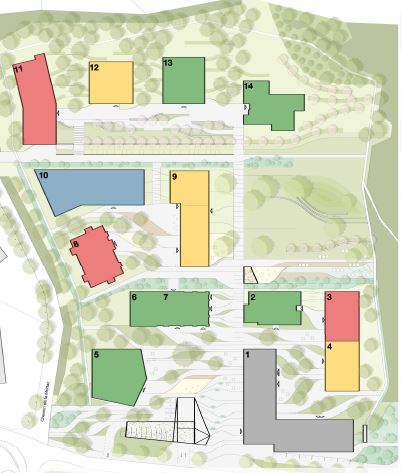
\includegraphics[width=0.45\textwidth]{ppa_buildings.JPG}
\caption{Map of the planned Eglantine district}
\label{fig:ppa_buildings}
\end{figure}

The energy profile of the buildings is calculated according to Minergie standard, as well as the SIA norms. Given the annual energy demand for space heating and hot water, as shown in Table \ref{tab:ppa_summary}, the monthly profile is shown in Figure \ref{fig:ppa_energydemand}.

\begin{figure}[htp]
\centering
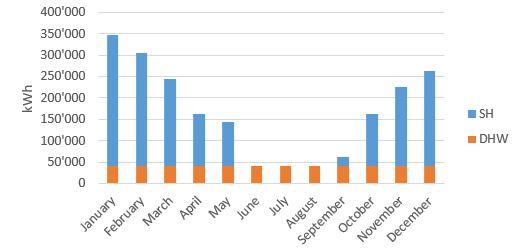
\includegraphics[width=0.7\textwidth]{ppa_energydemand.JPG}
\caption{Annual energy distribution for space heating and hot water}
\label{fig:ppa_energydemand}
\end{figure}

\subsubsection{Pre-studies}
Some pre-studies have been commissioned by the land-owner, in order to give, on an indicative basis, the sizing of the energy system. These studies have been realized by external engineering firms and the results are contained in the call for tender. The studied parameters include the sizing for heat pumps, geothermal wells, as well as PV, and are shown in Table \ref{tab:ppa_prestudy}. They estimate a PV potential on the building roofs of $570 kWp$, and the need for an installed heating power of $1'258 kW$, using 77 geothermal wells of an average length of $271 m$
\begin{table}[h!]
\centering
\caption{Estimated sizing of energy system in call for tender}\vspace{2mm}
\label{tab:ppa_prestudy} 
\begin{tabular}{lllll}
\toprule
\textbf{Building} & \textbf{PV}    & \textbf{HP}    & \multicolumn{2}{l}{\textbf{Geothermal}} \\
         &       &       & \textbf{Nb. wells}        & \textbf{Depth}        \\
         & \textbf{[kWp]} & \textbf{[kW] } &                 & \textbf{[m] }         \\
         \midrule
1        & 46    & 223   & 13              & 284          \\
2        & 45    & 70    & 4               & 291          \\
3        & 35    & 64    & 4               & 269          \\
4        & 33    & 76    & 5               & 250          \\
5        & 49    & 100   & 6               & 276          \\
6        & 55    & 41    & 3               & 225          \\
7        & 55    & 77    & 5               & 256          \\
8        & 37    & 68    & 4               & 281          \\
9        & 66    & 115   & 7               & 271          \\
10       & 0     & 121   & 7               & 286          \\
11       & 59    & 114   & 7               & 269          \\
12       & 33    & 63    & 4               & 259          \\
13       & 32    & 63    & 4               & 259          \\
14       & 27    & 63    & 4               & 267          \\
\midrule
\textbf{TOT}      & \textbf{570}   & \textbf{1'258} & \textbf{77}              &             \\
\bottomrule
\end{tabular}
\end{table}

\subsubsection{Calculations/Energy demand/Typical days}
\todo{write section eglantine calculations/energy demand}

\begin{itemize}
	\item typical days resulting profile
	\item cooling demand deduced from SIa or minergie
	\item ...
\end{itemize}

Figure \ref{fig:energyDemand}, including occurrencies. 

\begin{figure}[h!]
	\centering
	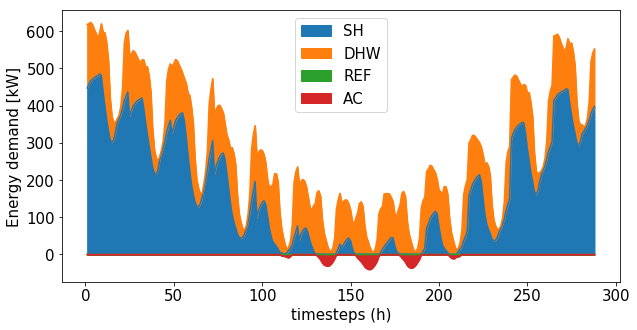
\includegraphics[width=0.7\textwidth]{energy_demand.png}
	\caption{Total energy demand of the Eglantine district}
	\label{fig:energyDemand}
\end{figure}


\subsection{Heat sources}
The heat pumps in a system can source heat from various sources. Depending on the case, it is more convenient to use one or the other, given the varying temperatures and investment costs.

\subsubsection{Stream}
A small stream flows along the eastern boundary of the area, on which the Eglantine district is being built. The official numbers of the canton Vaud \cite{veillehydro-meteorologiqueducantondevaudMorgesRiviereDebit} are shown in Figure \ref{fig:river}, in which the Temperature and the water flow are plotted. These values represent the average over a period of several years (7 for the temperature, and 12 for the flow rates). 

\begin{figure}[htp]
	\centering
	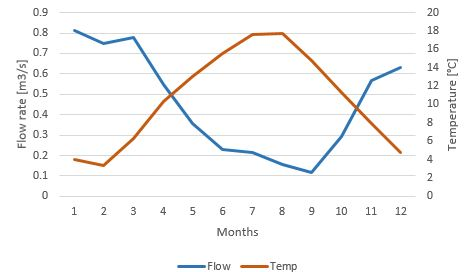
\includegraphics[width=0.5\textwidth]{river.JPG}
	\caption{Temperature and flow of the Morges river}
	\label{fig:river}
\end{figure}

According to this graph, it could be thought of using this river as a heat source for the heat pumps. However, what is not displayed is the minimum values. In fact, during droughts, the flow rate would not be sufficient to cover the heating/cooling demand. In fact, the lowest value has been reached in August 2004 with $0.017 m^3/s$, and even in December 2005 the lowest daily flow was of $0.057 m^3/s$. \\
For this reason, the stream has been excluded from further analysis and has not been considered as a viable solution.

\subsubsection{Lake}
Through a pipe, the water is pumped from the lake, at a depth of around 70 m, to the central plant, located in the district area. 

The massflow of the water is calculated in order to satisfy a drop/rise in the water stream of $\Delta T_{water}  = 4 \si{\celsius}$.

The cost function is calculated as for the CO2 pipes (see Section \ref{sss:net}), considering the needed diameter to satisfy the heating/cooling demand, which depend on the different heat capacity and massflow of the water.


\subsubsection{Geothermal wells}
The average temperature of a geothermal well is calculated according to Section \ref{ss:gtw}. The temperature gradient in the lemanic region is found in experimental data from the canton Geneva\cite{gadzEvaluationPotentielGeothermique2011}:
\begin{equation}
	\nabla T_{g} = 0.03 [K/m]
\end{equation}
This value also corresponds to the average gradient found in the Swiss plateau\cite{siaSIA384Sondes2010}.

The average surface temperature depends mainly on the latitude and on the altitude. Standard values for different regions of Switzerland can be found in the SIA norm 384\cite{siaSIA384Sondes2010}. Experimental measurements\cite{gadzEvaluationPotentielGeothermique2011} show that the surface temperature in the lemanic region is:\todo{add images of gradient and surface temperature from PGG report?}
\begin{equation}
	T_{g,s} = 11 \si{\celsius}
\end{equation}
Knowing the average depth of the geothermal wells, which is found to be $L_{gtw} = 267$ (see Section \ref{ss:Eglantine}), the mean temperature in the geothermal well corresponds to:
\begin{equation}
	T_{g, mean} = 15 \si{\celsius}
\end{equation}

It is assumed that the geothermal wells are well sized, in order to respect the natural recharge rate, which is strongly dependent on the type of soil. The sizing of the boreholes is very important to ensure a sustainable use of the ground heat throughout the years. \\

\begin{figure}[htp]
	\centering
	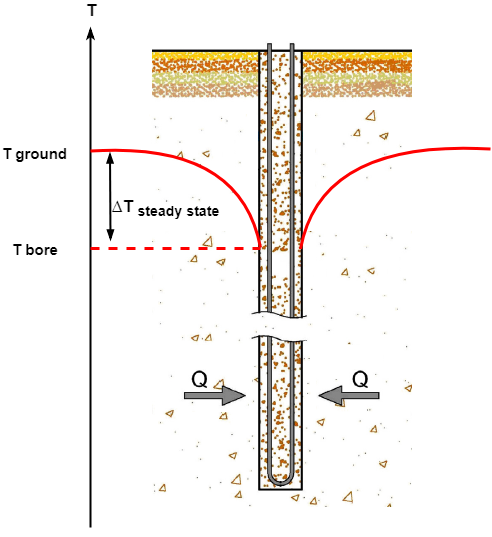
\includegraphics[width=0.5\textwidth]{GTW_T_profile.png}
	\caption{Steady state temperature difference in borehole, due to heat extraction}
	\label{fig:GTW_T}
\end{figure}

Nevertheless, there is a temperature gradient that will form around the borehole at any time heat is extracted, as shown in Figure \ref{fig:GTW_T}, in the steady state that depends of the heat extraction rate and the conductivity of the soil. This temperature difference ($\Delta T_{steady state}$) is assumed to be 3 \si{\celsius} \cite{guoTechnoeconomicComparisonDirect2012,hanSensitivityAnalysisVertical2016}.
Thus the mean useful temperature of the borehole over its depth is given by:
\begin{equation}
	T_{b, mean} = T_{g, mean} -\Delta T_{Steady State} = 12 \si{\celsius}
\end{equation}

The minimum approach temperature necessary to exchange heat with the soil can be determined with help of the procedure described in Section \ref{ss:dtmin}. 

The price for boreholes in Switzerland is found to be around $80 CHF/m$ \cite{bawos.chMitErdsondenbohrungenKosten2018}. 
Assuming a typical pipe diameter of $32 mm$\cite{siaSIA384Sondes2010, kruseStatusDevelopmentResearcha}, the corresponding cost of the heat exchange area of the borehole calculated.

To perform the $\Delta T_{min}$ optimization, the overall heat transfer coefficients of the well - including the fluid, the bore wall and the soil - are assumed to be\cite{kruseStatusDevelopmentResearcha}:
\begin{align}
	& U^{g/water} = 9.3 kW/m^2K
	& U^{g/CO2} = 17.1 kW/m^2K
\end{align}

The resulting minimum approach temperatures in ground heat exchanges are:
\begin{align}
	&\Delta T_{min}^{g/water} = 14 \si{\celsius}
	&\Delta T_{min}^{g/CO2} = 6.8 \si{\celsius}
\end{align}
These values are similar to experimental or standard values found in literature \cite{siaSIA384Sondes2010, lamarcheReviewMethodsEvaluate2010}.\\

The water rise/drop in the water ground loop is assumed to be $dT_{water} = 4 \si{\celsius}$ \cite{lundDESIGNCLOSEDLOOPGEOTHERMAL}\\


\todo{this cost function here?}
The price for boreholes in Switzerland is found to be around $c_{wells} = 80$ [CHF/m] \cite{bawos.chMitErdsondenbohrungenKosten2018}. 
In order to provide the model with an energy dependent cost function, this value is transformed with help of the data from Table \ref{tab:ppa_prestudy}:
\begin{align}
&  L_{wells}^{tot} = n_{wells} * L_{well}^{average} \\
& 	\text{Cost function [CHF/kW]} = c_{wells} \frac{L_{wells}^{tot}}{P_{hp}^{tot}}
\end{align}
where $L_{wells}$ is the length and $n_{wells}$ the number of boreholes, and $P_{hp}$ is the total power of heat pumps installed.\\

inv cost is given by the Qwinter-Qsummer
\subsection{External heat sources}
The main advantage of a 5th generation district heating network is the ability to recover heat, and exchange it among the diversity of user. In the case of the Eglantine project, inside the district there are only very small heat sources and it is thus necessary to identify potential heat sources, located in the surroundings. 
Two potential heat sources have been identified in the surroundings of the Eglantine district: the ice rink and a shopping mall.

\subsubsection{Ice rink}

\begin{figure}[htp]
	\centering
	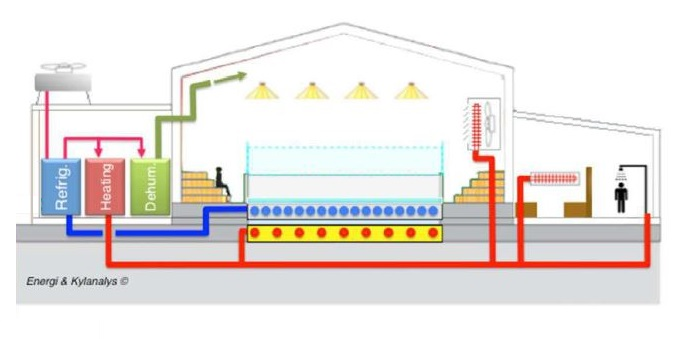
\includegraphics[width=1\textwidth]{IR_schema.JPG}
	\caption{Energy system of a typical ice rink \cite{gronqvistComparativeLifecycleCost}}
	\label{fig:IR_schema}
\end{figure}

An ice rink is a place where people can ice skate and play winter sports. The ice surface is normally inside an arena, which ensures comfortable temperatures for the people on the ice, as well as for the public, throughout the season. This also allows to extend the season, avoiding ice melt, when temperatures are warmer outside.\\

A study, conducted on more than one hundred ice rinks in Sweden, shows that the refrigeration system used to cool the ice surface has the largest share in total energy consumption, 43\% (in average) as indicated in Figure \ref{fig:IR_energyDemand} \cite{karampourMEASUREMENTMODELLINGICE}. 
However, the ice rink often also includes changing rooms with showers, and a cafeteria or a restaurant, which also present heating demand. According to Figure \ref{fig:IR_energyDemand}, the average share of heating in the total energy demand is 26\%.
Last but not least, the ice surface has to be constantly illuminated, which requires a powerful lightning system. The global system is shown in Figure \ref{fig:IR_schema}.\\

However, for practicality reasons, it is assumed that only the refrigeration system is connected to the CO2 network, while the heating and electricity demand is supplied by the existing system, and are thus not considered in this model.

\begin{figure}[htp]
	\centering
	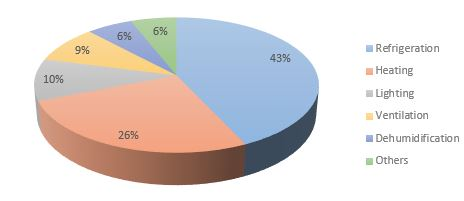
\includegraphics[width=0.7\textwidth]{IR_energyDemand.JPG}
	\caption{Energy demand of a typical ice rink \cite{karampourMEASUREMENTMODELLINGICE}}
	\label{fig:IR_energyDemand}
\end{figure}

Ice rinks are conventionally cooled with indirect systems, as shown in the right part of Figure \ref{fig:IR_refSystem}, based on a ammonia (NH3) vapor compression chiller, exchanging with a secondary brine loop that extracts the heat from the ice surface. The waste heat is normally, or at least in older systems, exchanged with the environment, with help of cooling towers. Connecting it to a 5th generation district heating network, would allow recovering this heat and use it to cover the heat demand of other users. The connection to the CO2 network is shown in the left part of Figure \ref{fig:IR_refSystem}.\\

This presents a high energy and exergy efficiency gain, since the refrigeration system can be driven on a lower and constant condensation temperature.
\todo{insert equations for temperatures with dTmins?}

\begin{figure}[htp]
	\centering
	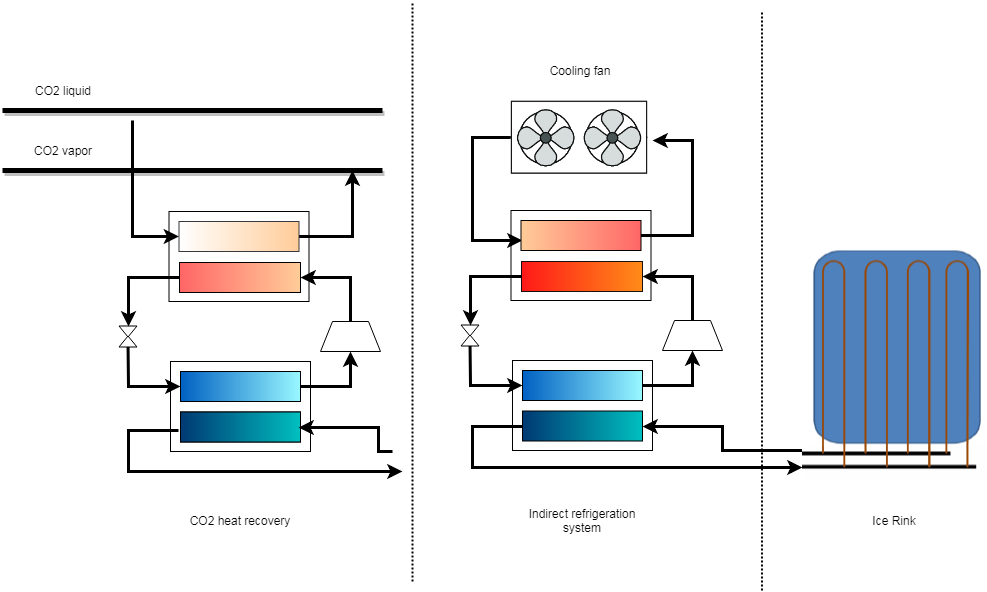
\includegraphics[width=1\textwidth]{IceRink_refrigeration.png}
	\caption{Refrigeration systems for ice rinks}
	\label{fig:IR_refSystem}
\end{figure}

The calculation of the cooling demand of the ice rink is based on the following assumptions:
\begin{itemize}
	\item Constant load profile throughout the ice season
	\item Ice season: 1st of August - 1st of April
	\item $COP_{ref} = 4$ \cite{karampourMEASUREMENTMODELLINGICE}
	\item Total waste heat = $ 450 MWh/year$ \cite{kolasniewskiEvaluationModellingIce}
	\item $dT_{min}(refrigerant-ice) = 1 \si{\celsius}$
	\item $dT_{min}(refrigerant-refrigerant) = 3 \si{\celsius}$
\end{itemize}

The daily cooling demand profile of the ice rink, is based on the required ice temperature, which varies throughout the day\cite{karampourMEASUREMENTMODELLINGICE}, as shown in Table \ref{tab:IR_profile}.

\begin{table}[h]
\centering
\label{tab:IR_profile}
\caption{Ice rink refrigeration profile}\vspace{2mm} 
\begin{tabular}{lll}
\toprule
\textbf{Period} & \textbf{Rink function} & \textbf{\begin{tabular}[c]{@{}l@{}}$T_{ice}$\\ {[}\si{\celsius}{]}\end{tabular}} \\
\midrule 
0.00-6:00   & Night setback   & -1     \\
6:00-8:00   & Ice maintenance & -1     \\
8:00-16:00  & Low load        & -3     \\
16:00-18:00 & Figure skating  & -4     \\
18:00-24:00 & Hockey          & -6    \\
\bottomrule
\end{tabular}
\end{table}

Thus the computed energy demand is shown in Figure...
\missingfigure{add figure with load profile}

%\begin{figure}[h!]
%	\centering
%	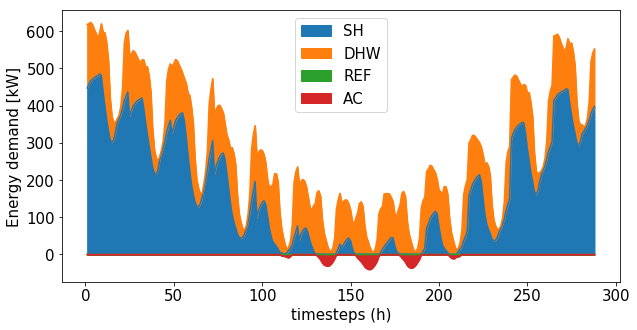
\includegraphics[width=0.7\textwidth]{energy_demand.png}
%	\caption{Total energy demand of the Eglantine district}
%	\label{fig:energyDemand}
%\end{figure}

The refrigeration system is modeled the same way as in the reference scenario, taking the lower heat delivery temperatures into account.

\subsubsection{Shopping mall}

\subsection{Variants / Scenarios}

\subsubsection{Heating}
The heating demand is supplied by a set of decentralized geothermal heat pumps, one for domestic hot water and one for space heating in every building. These heat pumps source the ambient heat from a secondary loop that exchanges heat with the ground through a system of geothermal wells, the SL-GSHP, which is described in Section \ref{ss:dx}. 

Given the relevance of the heat pumps in the studied energy system, it has been chosen to use its thermodynamic model, which achieves more reliable and precise results.\\

The temperatures at the evaporator and condenser are given by the following equations:
\begin{equation}
T_{evap} = T_{ground} - \Delta T_{min}^{ground/water} - \Delta T_{water} - \Delta T_{min}^{ref/water}
\end{equation}
\begin{equation}
T_{cond} = T_{demand} + \Delta T_{min}^{ref/water}
\end{equation}
where $\Delta T_{min}$ are the corresponding minimum approach temperatures, and $\Delta T_{water}$ is the temperature rise in the secondary water loop exchanging with the ground.

For the space heating heat pump, the refrigerant used is R123yf, as described in Section \ref{sss:hp_thermo}.\\

For the domestic hot water, it is chosen to use transcritical CO2 heat pumps. As described in Section \ref{sss:hp_CO2}, this technology can achieve very good performances supplying heat that requires a high lift. This is the case in domestic hot water, where the water has to be heated from a temperature of 10 \si{\celsius} to a temperature of 55 \si{\celsius}.

\subsubsection{Cooling}
Given the availability of geothermal wells, it has been chosen to implement geo-cooling for space cooling. The system is providing cooling at the ground temperature, corrected with the minimum approach temperature $\Delta Tmin_{ground/water}$ and the temperature rise in the water loop $\Delta T_{water}$.
\begin{equation}
T_{geo-cooling} = T_{ground} + \Delta T_{min}^{ground/water} + \Delta T_{water}
\end{equation}

\subsubsection{Refrigeration}
The refrigeration is achieved with a set of decentralized air cooled vapor compression chillers, which present the same working principle as heat pumps. Given that energy demand for refrigeration is not as relevant in the case study, it has been chosen to use the basic Carnot cycle model, as explained in Section \ref{sss:hp_carnot}. The heat is evacuated into the environment with help of cooling towers, as described in Section \ref{sss:cooling_tower}.

Thus, the total energy consumption is a sum of the energy demand of the compressor and the cooling fans.
\begin{equation}
\dot{E} = \dot{E}_{ref} + \dot{E}_{fans}
\end{equation}

and the operating temperatures are defined in the following way:
\begin{equation}
T_{cond} = T_{ext} + \Delta T_{air} + \Delta T_{min}^{ref/air}
\end{equation}
where $\Delta T_{air}$ is the temperature difference of the cooling air between the input and the output of the condenser, while $\Delta T_{min}^{ref/air}$ is the minimum approach temperature difference needed for heat transfer between a refrigerant and air.\\


\subsection{Reference scenario}
In order to evaluate the potential of alternative energy systems, a reference scenario is defined. Data about the energy system that will be built in the Eglantine district is not available to the author, and therefore a standard state of the art system is used. It is assumed that the heat demand for space heating and domestic hot water is provided by decentralized geothermal sourced heat pumps. The cooling demand is provided by air cooled vapor 

 chillers, also commonly known as air conditioners. The scenario foresees the installation of PV panels on the roof of the buildings.

\missingfigure{energy schema ref scenario}

The main resource flows are shown in Table \ref{tab:layers_ref}.
\begin{table}[h!]
	\centering
	\caption{Resource flows for the reference energy system ((-): flow in / (+): flow out))}\vspace{2mm}
	\label{tab:layers_ref} 
	\begin{tabular}{lccc}
		\toprule
		& \multicolumn{3}{c}{Resource flows}             \\
		Units          & Electricity & $Source_{hot}$ & $Source_{cold}$ \\ \midrule
		$HP_{sh}$      & -           & -              & +               \\
		$HP_{dhw}$     & -           & -              & +               \\
		$HP_{ref}$     & -           & +              & -               \\
		$HE_{ac}$      &             & +              & -               \\
		Elec. Heater   & -           &                &                 \\
		PV             & +           &                &                 \\
		$GTW_{winter}$ &             & +              & -               \\
		$GTW_{summer}$ &             & -              & +              \\ \bottomrule
	\end{tabular}
\end{table}


\subsubsection{Heating}
The heating demand is supplied by a set of decentralized geothermal heat pumps, one for domestic hot water and one for space heating in every building. These heat pumps source the ambient heat from a secondary loop that exchanges heat with the ground through a system of geothermal wells, the SL-GSHP, which is described in Section \ref{ss:dx}. 

Given the relevance of the heat pumps in the studied energy system, it has been chosen to use its thermodynamic model, which achieves more reliable and precise results.\\

The temperatures at the evaporator and condenser are given by the following equations:
\begin{equation}
    T_{evap} = T_{ground} - \Delta T_{min}^{ground/water} - \Delta T_{water} - \Delta T_{min}^{ref/water}
\end{equation}
\begin{equation}
    T_{cond} = T_{demand} + \Delta T_{min}^{ref/water}
\end{equation}
where $\Delta T_{min}$ are the corresponding minimum approach temperatures, and $\Delta T_{water}$ is the temperature rise in the secondary water loop exchanging with the ground.

For the space heating heat pump, the refrigerant used is R123yf, as described in Section \ref{sss:hp_thermo}.\\

For the domestic hot water, it is chosen to use transcritical CO2 heat pumps. As described in Section \ref{sss:hp_CO2}, this technology can achieve very good performances supplying heat that requires a high lift. This is the case in domestic hot water, where the water has to be heated from a temperature of 10 \si{\celsius} to a temperature of 55 \si{\celsius}.

\subsubsection{Cooling}
Given the availability of geothermal wells, it has been chosen to implement geo-cooling for space cooling. The system is providing cooling at the ground temperature, corrected with the minimum approach temperature $\Delta Tmin_{ground/water}$ and the temperature rise in the water loop $\Delta T_{water}$.
\begin{equation}
T_{geo-cooling} = T_{ground} + \Delta T_{min}^{ground/water} + \Delta T_{water}
\end{equation}

\subsubsection{Refrigeration}
The refrigeration is achieved with a set of decentralized air cooled vapor compression chillers, which present the same working principle as heat pumps. Given that energy demand for refrigeration is not as relevant in the case study, it has been chosen to use the basic Carnot cycle model, as explained in Section \ref{sss:hp_carnot}. The heat is evacuated into the environment with help of cooling towers, as described in Section \ref{sss:cooling_tower}.

Thus, the total energy consumption is a sum of the energy demand of the compressor and the cooling fans.
\begin{equation}
\dot{E} = \dot{E}_{ref} + \dot{E}_{fans}
\end{equation}

and the operating temperatures are defined in the following way:
\begin{equation}
    T_{cond} = T_{ext} + \Delta T_{air} + \Delta T_{min}^{ref/air}
\end{equation}
where $\Delta T_{air}$ is the temperature difference of the cooling air between the input and the output of the condenser, while $\Delta T_{min}^{ref/air}$ is the minimum approach temperature difference needed for heat transfer between a refrigerant and air.\\

\subsection{CO2 DEN}
CO2 network energy system showed in Figure...
\missingfigure{energy syst schema CO2 DEN}

The main resource flows are shown in Table \ref{tab:layers_CO2}.
\begin{table}[h!]
	\centering
	\caption{Resource flows for the CO2 DEN ((-): flow in / (+): flow out))}\vspace{2mm}
	\label{tab:layers_CO2} 
	\begin{tabular}{llllll}
		\multicolumn{1}{c}{-} & \multicolumn{5}{c}{Resource flows}                                          \\
		Units                 & Electricity & $CO2_{liq}$ & $CO2_{vap}$ & $Source_{hot}$ & $Source_{cold}$ \\
		$HP_{cp}^{winter}$    & -           & -           & +           & -              & +               \\
		$HP_{cp}^{summer}$    &             & +           & -           & +              & -               \\
		$HP_{sh}$             & -           & +           & -           &                &                 \\
		$HP_{dhw}$            & -           & +           & -           &                &                 \\
		$HP_{ref}$            & -           & -           & +           &                &                 \\
		$HE_{ac}$             &             & -           & +           &                &                 \\
		Elec. Heater          & -           &             &             &                &                 \\
		PV                    & +           &             &             &                &                 \\
		$GTW_{winter}$        &             &             &             & +              & -               \\
		$GTW_{summer}$        &             &             &             & -              & +              
	\end{tabular}
\end{table}


\subsubsection{Heating}
For space heating and domestic hot water, the same model as for the heat pumps in reference scenario are used. Sicne in this case the HP sources heat from the CO2 network instead of the geothermal wells, the mayor difference lies in the evaporation temperature, which corresponds to temperatuer in the CO2 vapor pipe ($T_{CO2,g}$):
\begin{equation}
    T_{evap} = T_{CO2,g} - \Delta T_{min}^{ref/ref}
\end{equation}

\subsubsection{Refrigeration}
As for the reference scenario, refrigeration is achieved through decentralized vapor compression chillers. However, in this case they are not air cooled, but they exchange directly with the CO2 network. Thus, the temperature in the condenser is given by:
\begin{equation}
    T_{cond} = T_{CO2,l} + \Delta T_{min}^{ref/CO2}
\end{equation}

\subsubsection{Cooling}
Free cooling has been modeled by a simple heat exchanger that evaporates saturated liquid CO2, which is then injected back into the network in a superheated vapor state with $\Delta T_{superheating} = 1K$. The mass flow of the CO2 is adapted to satisfy the cooling demand. It is assumed that pressure and temperature losses are negligible.

\subsubsection{Central plant}
As mentioned before, for obvious reasons, heating and cooling loads in the system are not always balanced. Thus, there is the need for a central plant to balance out the system, able to heat and cool. A centralized heat pump is very suitable for this purpose.

Equations and modeling are the same as for the above described heat pumps. Difference consists in heat source, and thus evaporation temperature. Different options have been studied:
\begin{itemize}
    \item River: as for the lake, river water can be an interesting source of heat, with the difference of seasonal fluctuations. During the winter, river water can have a temperature close to 0, while in the summer it can rise to more than 20 \si{\celsius}. In the case of the Eglantine district, there is a small stream, called Morges, that passes at the eastern border of the land.
    \item Lake: sourced from a certain depth, lake water shows an almost constant temperature of around 7.5 \si{\celsius} throughout the year. This solution can be very interesting alternative to geothermal wells, since, if close enough, it might reduce the upfront costs, despite probably slightly increasing the operating costs. In this particular case, the distance to the lake is of 1500 m.
    \item Geothermal wells: after a certain depth, the ground presents a constant and very interesting temperature throughout the year. This heat can be exchanged with help of a secondary loop or through direct expansion of the refrigerant into the ground coils.
\end{itemize}

\todo{explain lake=ref, geoth=DHX CO2}
Direct expansion system is assumed (see Section \ref{ss:dx}).
So the CO2 DEN with DX-GSHP technology is shown in Figure \ref{fig:co2_gshp}

\begin{figure}[htp]
	\centering
	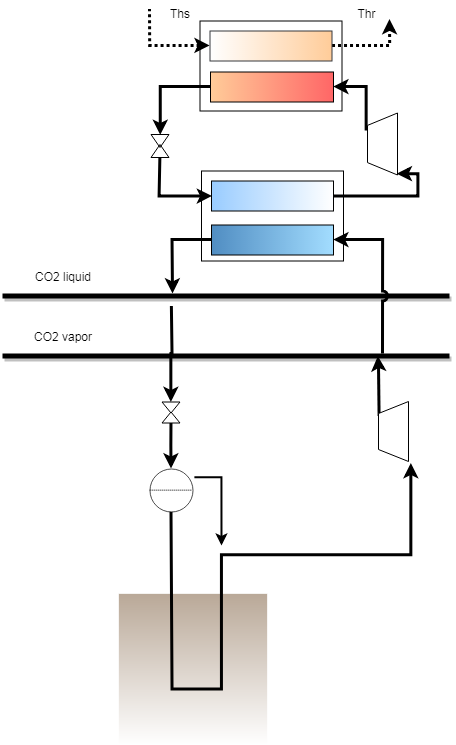
\includegraphics[width=0.3\textwidth]{CO2-DX-GSHP.png}
	\caption{A simplified schematics of the CO2 DEN with DX-GSHP technology}
	\label{fig:co2_gshp}
\end{figure}

The operating temperatures are calculating the following way.
\begin{equation}
    T_{evap} = T_{source} - \Delta T_{min}^{CO2/source}
\end{equation}
The operating pressure is calculated with help of \textit{Coolprop}. The results are shown in Table \ref{tab:cp_source}.
\begin{table}[h!]
\centering
\caption{Operating conditions for direct expansion of CO2 in heat source}\vspace{2mm}
\label{tab:cp_source} 
\begin{tabular}{lllll}
\toprule
\textbf{Source}     & \textbf{\begin{tabular}[c]{@{}l@{}}$\Delta T_{min}^{ref/source}$\\ $[\si{\celsius}]$\end{tabular}} & \textbf{\begin{tabular}[c]{@{}l@{}}$T_{source}$\\ $[\si{\celsius}]$\end{tabular}} & \textbf{\begin{tabular}[c]{@{}l@{}}$T_{evap}$\\ $[\si{\celsius}]$\end{tabular}} & \textbf{\begin{tabular}[c]{@{}l@{}}$P_{CO2}$\\ $[bar]$\end{tabular}} \\
\midrule
\textbf{Lake}       & 4                                                                                     & 7.5                                                                  & 3.5                                                                & 38.2                                                               \\
\textbf{Geothermal} & 10                                                                                    & 11                                                                   & 1                                                                  & 35.8     \\
\bottomrule
\end{tabular}
\end{table}
\todo{summary table needed here (Ts, dTmin, Tevap, P...)? wrong values now}


\subsection{Values/typical days/...}
\todo{Table with values}
\begin{itemize}
	\item cinv
	\item cel-/+
	\item cop: In this project, cop1 (fixed) value is assumed to be negligible.
	\item dtmin
	\item with respectively 1 and 2 \si{\celsius} of superheating and subcooling at the outlet of the heat exchanger \cite{}.\todo{missing reference for superheat and subcool temp}
	\item ...
\end{itemize}

\subsubsection{Investment cost functions}

As described in Section \ref{ss:osmose}, the model need investment cost parameters that can be calculated with the procedure explained in Section \ref{ss:ic}.

Values for the heat pumps are given in Henchoz et al., obtained by linearizing commercial products\cite{henchozPerformanceProfitabilityPerspectives2015}. The cost function for heat exchangers has been interpolated in order to have a function dependent on the amount of exchanged heat.

\begin{table}[htp]
	\centering
	\caption{Summary of the the investment cost function of each technology, including their expected lifetime and the interest rate.}
	\label{tab:ic}
\begin{tabular}{lcccc} \toprule
	\textbf{Technology} & Cost function [Euro] & X  [unit]       & Interest rate & Lifetime \\ \midrule
	HP                  & 1'240 X + 5680       & $E_{comp}$ [kW] & 0.08                              & 20                           \\
	heat exchanger      & 215 X + 56          & $Q$ [kW]        & 0.08                              & 20                           \\
 	Electric heater		& 23 X + 968		  &	$Q$ [kW] 		 & 0.08								& 20						   \\
	PV                  & 300 X                & A [$m^{2}$]     & 0.08                              & 20                           \\
	Geothermal wells    & 2890 X + 5800        & $Q$ [kW]        & 0.03                              & 50                  			 \\
	Network				& See Section \ref{sss:net}		&		 &									 &					    \\ \bottomrule     
\end{tabular}
\end{table}

Values are summarized in Table \ref{tab:ic}.

\subsubsection{Minimum approach temperature}
As seen in Table \ref{tab:alphas}, CO2 (R744) has a higher heat transfer coefficient than other conventional refrigerants, as for example R1234yf. This has to be taken into account in the energy system through a different minimum approach temperature. To do so, there are two possible approaches:
\begin{itemize}
	\item calculate a new, lower, $\Delta T_{min}^{R744}$, maintaining the same heat exchange area $A_{ex}$. This results in higher COP for the heat pump and thus lower operating costs $OC_{hp}$
	\item calculate a new, smaller, heat exchange area  $A_{ex}$, maintaining the same $\Delta T_{min}$. This leads to lower upfront costs $IC_{ex}$
\end{itemize}

It is chosen to use different $\Delta T_{min}^{R744}$, maintaining the same heat exchange area. The following procedure is repeated for the various fluids ($X$) the refrigerants have to exchange with:
\begin{enumerate}
	\item Calculate $U_{R1234yf/X}$ with Equation \ref{eq:alpha}
	\item Optimize $\Delta T_{min}^{R1234yf/X}$ with numerical values from the Eglantine district, as described in Section \ref{ss:dtmin}
	\item Calculate  $U_{R744/X}$ 
	\item Solve Equation \ref{eq:HEX_area} in function of $\Delta T$, using $U_{R744/X}$ and the $A_{ex}$ resulting from the previous step.
\end{enumerate}

The implementation of this algorithm has been solved on \textit{Matlab} with help of function \textit{solve(equation \ref{eq:HEX_area}, $\Delta T_{min}$)}.
Thus resulting $\Delta T_{min}$ values shown in Table \ref{tab:dtmins}.

\begin{table}[h!]
\centering
\caption{Minimum approach temperatures used for heat exchanges in the model}\vspace{2mm}
\label{tab:dtmins} 
\begin{tabular}{lllll}
\toprule
	$\Delta T_{min}$ [K] & Ground & Water & R744 & R1234yf \\
	Water                & 14     & -     & -    & -       \\
	R744                 & 6.8    & 3.46  & 0.8  & -       \\
	R1234yf              & -      & 4     & 1.4  & 2.3    \\ \bottomrule
\end{tabular}
\end{table}


As example, Figure \ref{fig:dtmin_wr} and Figure \ref{fig:dtmin_gtw} show the resulting optimization of the minimum approach temperatures, respectively for refrigerant and ground heat exchanges. The straight line shows the optimum $\Delta T_{min}$ for the reference heat exchange, in function of the total costs (green line), while the dashed line shows the improved $\Delta T_{min}$ for CO2, maintaining the same $A_{ex}$.

\begin{figure}[!htb]
	\centering
	\begin{minipage}{.45\textwidth}
		\centering
		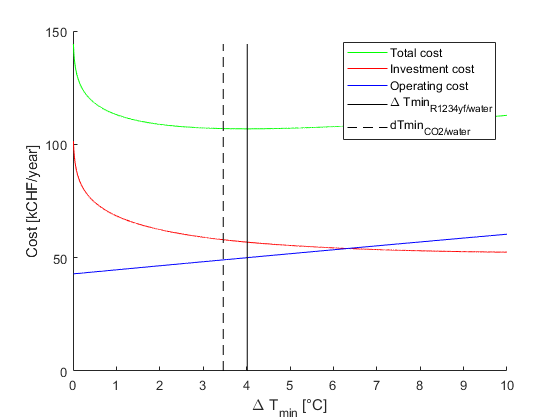
\includegraphics[width=\linewidth]{dtmin_wr}
		\caption{Optimization of $\Delta T_{min}$ values for heat exchange with refrigerant R1234yf, through minimization of total costs (green line)}
		\label{fig:dtmin_wr}
	\end{minipage}%
	\hspace{1cm}
	\begin{minipage}{0.45\textwidth}
		\centering
		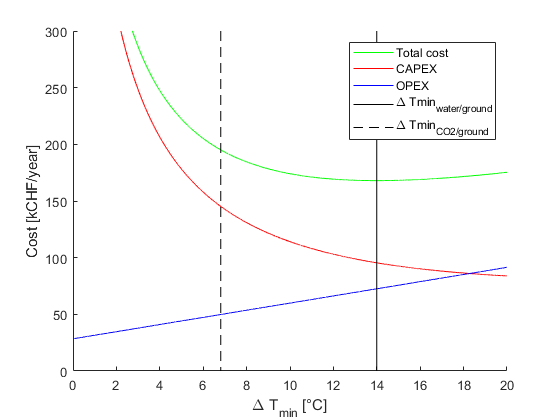
\includegraphics[width=\linewidth]{dtmin_gtw}
		\caption{Optimization of $\Delta T_{min}$ values for heat exchange with the ground, through minimization of total costs (green line)}
		\label{fig:dtmin_gtw}
	\end{minipage}
\end{figure}

\subsubsection{Compressor efficiencies}
The compressor efficiencies are directly calculated in the model, according to the equations in Section \ref{sss:hp_CO2} and \ref{sss:hp_thermo}. could be directly implemented in model. Table \ref{tab:eta_comp} shows the resulting efficiencies in standard operating conditions, for the different heat pumps used in this work.

\begin{table}[h!]
	\centering
	\caption{Calculated efficiencies for heat pump compressors, during the average day in January}\vspace{2mm}
	\label{tab:eta_comp} 
\begin{tabular}{l@{\hskip 0.5in}lllll@{\hskip 0.5in}lll} \toprule
	-             & \multicolumn{5}{c}{CO2 DEN}            & \multicolumn{3}{c}{Reference scenario} \\
	Unit          & CP     & CP   & SH     & DHW  & REF    & SH           & DHW       & REF         \\
	Refrigerant   & R123yf & CO2  & R123yf & R744 & R123yf & R123yf       & R744      & R123yf      \\ \midrule
	$P_{d}$       & 5.0    & 43.0 & 9.4    & 84.9 & 5.0    & 9.4          & 66.0      & 11          \\
	$P_{s}$       & 2.4    & 20.2 & 4.6    & 46.7 & 2.80   & 2.4          & 30.4      & 2.4         \\
	$\eta_{mech}$ & 0.85   & 0.80 & 0.85   & 0.78 & 0.85   & 0.85         & 0.80      & 0.85        \\
	$\eta_{is}$   & 0.85   & 0.70 & 0.85   & 0.71 & 0.85   & 0.82         & 0.70      & 0.81        \\
	$\eta_{comp}$ & 0.72   & 0.56 & 0.72   & 0.55 & 0.72   & 0.70         & 0.56      & 0.69       \\ \bottomrule
\end{tabular}
\end{table}

These values are similar to reference values found by Yang et al.\cite{yangTheoreticalExperimentalInvestigation2016} in their experimental work.


%\subsection{Analysis/Extrapolation scenario}
%A scenario to study parameters independently from Eglantine.
%Parameters to study/extrapolate for quick application on other districts:
%\begin{itemize}
%    \item influence on IC,OC,TC
%    \item influence on network temperature $T_net$  
%\end{itemize}
%Varying \% of cooling load, wrt heating load, using varying composition of cities, with categories (commercial/residential/...)

\subsection{CP with if conditions}
\todo{not sure where to put that...}
In order to have a HP model for the central plant, which is able to handle different source temperatures, different cases have been implemented, with help of if conditions. Indeed, computation problems arise when the source temperatures reaches the condensation temperature of the heating part of the CP, which corresponds to the temperature of the CO2 network. In the same way, this higher source temperature also precludes the possibility of free-cooling. However, if the temperatures is higher than the CO2 network, the central pump might be able to source heat without operating a heat pump (free-heating).

The model includes two operating modes for each part of the central plant, the heating part (CP-winter) and the cooling part (CP-summer). The thresholds are set in the following way:
\begin{align}
	& T_{thresh}^{free-cooling} = T_{CO2} - \Delta T \\
	& T_{thresh}^{free-heating} = T_{CO2} + \Delta T 
\end{align}
where $\Delta T$ is the minimum temperature difference needed for the specific heat exchange.

The truth table is shown in Table \ref{tab:CP_tt}.
\begin{table}[h!]
	\centering
	\caption{Truth table to determine if the CP operates in heat pump (HP) or in heat exchanger (HE) mode, depending on the borehole temperature and the threshold temperatures for free-cooling $T^{FC}$ and free-heating $T^{FH}$}\vspace{2mm}
	\label{tab:CP_tt} 
\begin{tabular}{lccc} \toprule
	$T_{borehole}$ & $\leq T^{FC}$ & $T^{FC} \leq T \leq T^{FH}$ & $\geq T^{FH}$ \\ \midrule
	CP-winter      & HP                             & HP                                                           & HE                             \\
	CP-summer      & HE                             & HP                                                           & HP                          \\ \bottomrule  
\end{tabular}
\end{table}

The parameters that vary through the if conditions are the electricity consumed $E_{cp}$ and the investment cost parameters. 

\subsection{DX Vs. SL-GSHP}
As discussed in Section \ref{ss:dx}, there is the possibility to directly expand the CO2 into the geothermal well, instead of exchanging with help of a secondary water loop. The different temperature levels are shown in Figure \ref{fig:Qt_dx}. 

Results of simulation, show the difference in performance, \ref{tab:dxVSsl}.

\begin{table}[htp]
\centering
\caption{Comparison of simulation results for a SL-GSHP, versus a DX-GSHP}\vspace{2mm}
\label{tab:dxVSsl} 
\begin{tabular}{lll}
	\toprule
	-                 & \begin{tabular}[c]{@{}l@{}}SL-GSHP\\ R1234yf\end{tabular} & \begin{tabular}[c]{@{}l@{}}DX-GSHP\\ R744\end{tabular} \\ \midrule
	$T_{source}^{lm}$ & 13                                                        & 13                                                     \\
	$T_{demand}^{lm}$ & 14                                                        & 14                                                     \\
	$T_{cond}^{lm}$   & 16.4                                                      & 15.8                                                   \\
	$T_{evap}^{lm}$   & -7                                                        & 8.2                                                    \\
	$COP_{real}$      & 6.5                                                       & 15.8                                                   \\
	$\eta_{COP}$   & ?                                  	                      & ?	                                                    \\
	$\eta_{exergy}$    & ?                                                         & ?   \\ \bottomrule                                                  
\end{tabular}
\end{table}


CO2 heat pump has lower efficiencies (see Table \ref{tab:eta_comp}) thus $\eta_{COP}$ but much lower temperature difference to cover. Thus, its real coefficient of performance, as well as the exergy efficiency, are clearly higher than for the SL-GSHP. In fact, the DX-GSHP results being about twice as good.

\begin{figure}[htp]
	\centering
	\includegraphics[width=0.6\textwidth]{Qt_dx.png}
	\caption{Schematic representation of heat exchanges and minimum approach temperatures for the central plant HP, comparing SL- and DX-GSHP}
	\label{fig:Qt_dx}
\end{figure}

It has to be noted that this specific heat pump globally presents very low  exergy values. This is due to ratio between the relatively high minimum approach temperatures and the very low temperature difference between the source temperature $T_{b}$ and the heat demand temperature $T_{vap}^{CO2}$.

\subsection{Model improvement - thermodyn cycle}
\todo{do i maintain results with simple cycles somewhere in the results to show how much better it is with cycle?}

Comparison of results with simple Carnot model and with thermodyn model. Show difference in COPs\\

Recalculation of $\eta_{COP}$ for all ETs. From the real COP calculated with help of coolprop and the thermodynamic cycle of the heat pump, the COP efficiency can easily be calculated
\begin{equation}
\eta_{COP} = \frac{COP_{real}}{COP_{theoretical}}
\end{equation}

Table with new eta cop values.\\

COP Comparison with values from literature?\\

%with Coolprop CO2 transcritical cycle calculator COP ~= 5 (4.94-5.13) for $T_evap$ = 2deg and 8.5 (8.36-8.78) with $T_evap$ = 13deg
%isentropic efficiency expansion valve = 0.8\cite{yangTheoreticalExperimentalInvestigation2016}


\section{Results and discussion}

\subsection{Variants}

\begin{enumerate}
	\item GS-HP: decentralized ground sourced heat pumps
	\item GS-CO2DEN: CO2 DEN with ground sourced central plant
	\item LS-CO2DEN: CO2 DEN with lake sourced central plant
\end{enumerate}

\subsubsection{Reference energy system}
A parametric optimization of the costs of the reference energy system (GS-HP) is shown in Figure \ref{fig:V_G_PO}.

It can be seen that the biggest difference in investment and operating cost is due to the sizing of the PV. In fact, when constraining the investment costs, the model installs only a small share of PV, which increases the operational costs. On the contrary, a high share of PV increases the systems rate of auto-sufficiency, lowering the operational costs. 

On the far right, the maximum allowed share of photovoltaic (PV) - set to twice the total roof area, which accounts for potential facades and free space PV - is reached. The operational are lowered thanks to a different handling of peak consumption. The optimal system installs a small share of electrical heater (R-EL) to cover peak demand, which allows to optimally size the heating heat pumps (HP-S, HP-DHW). In the last column on the right, the system chose not to install the electrical heater but installing larger heat pumps, which strongly increases upfront costs, but allows to further reduce the operational costs.

On the far left, the opposite phenomenon happens. To reduce upfront costs, the system chose to cover the heat demand almost entirely with help of the electric heater (R-EL), minimizing the size of the heating heat pumps (HP-SH, HP-DHW).

The optimum, with respect to the total cost of the energy system, is in the very middle of the graph, between column 2 and 3. The optimum is analyzed in the following chapters.

\begin{figure}[htp]
	\centering
	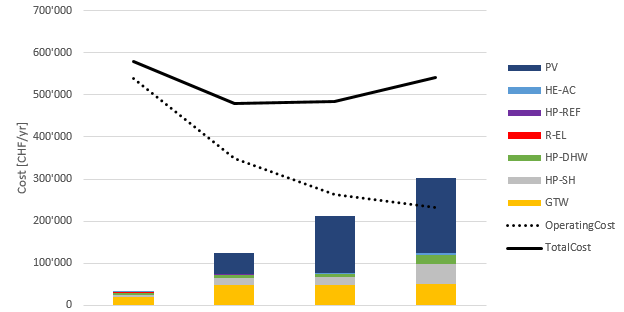
\includegraphics[width=1\textwidth]{V_G_PO1.png}
	\caption{Parametric optimization of the reference energy system (GS-HP), showing the detailed investment costs, the operational cost and the total cost}
	\label{fig:V_G_PO}
\end{figure}

\subsubsection{CO2 DEN on geothermal wells}
A parametric optimization of the costs of the CO2 district energy system with ground sourced central plant (GS-CO2DEN) is shown in Figure \ref{fig:V_CO2_G_PO}.

The response of this system to the parametric optimization is very similar to the one of the GS-HP system. This means that the biggest difference in investment and operating cost is due to the sizing of the PV, while the extreme cases are determined by the ration between the electrical heater (R-EL) and the heating heat pumps (HP-SH, HP-DHW).

Also in this case the lowest total cost of the energy system is to be found in the very middle of the graph, between column 2 and 3. The optimum is analyzed in the following chapters.

\begin{figure}[htp]
	\centering
	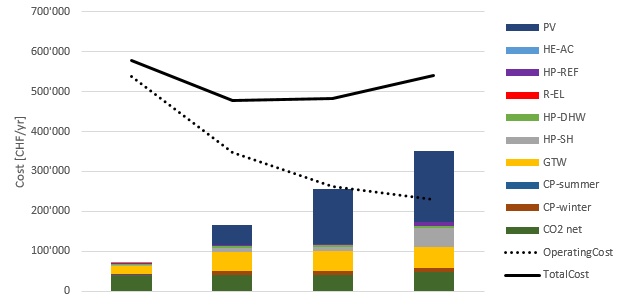
\includegraphics[width=1\textwidth]{V_CO2_G_PO1.png}
	\caption{Parametric optimization of the ground sourced CO2 DEN (GS-CO2DEN), showing the detailed investment costs, the operational cost and the total cost}
	\label{fig:V_CO2_G_PO}
\end{figure}

If we take the stable middle, isolate PV costs we obtain a share of network and HP correposnding to... This is shown in  Table \ref{tab:anergynets_IC}, in comparison with existing anergy networks in Switzerland.

\begin{table}[h!]
\centering
\caption{Cost comparison with existing anergy systems}\vspace{2mm}
\label{tab:anergynets_IC} 
\begin{tabular}{llrrr}  \toprule
	&          & Eglantine & \begin{tabular}[c]{@{}l@{}}Anergienetz \\ ETH Hönggerberg\end{tabular} & \begin{tabular}[c]{@{}l@{}}Anergienetz \\ Friesenberg\end{tabular} \\ \midrule
	$IC_{NET}$             & [\%]     & 33.6 \%    & 15.7 \%                                                                 & 25.9 \%                                                             \\
	$IC_{GTW}$             & [\%]     & 44.6 \%    & 32.7 \%                                                                 & 23.5 \%                                                             \\
	$IC_{Heating/Cooling}$ & [\%]     & 21.8 \%    & 49.2 \%                                                                 & 50.6 \%                                                             \\
	Heating power          & [kW]     & 592       & 8'000                                                                  & 3'930                                                              \\
	Heating demand         & [MWh/yr] & 2'390     & 28'450                                                                 & 35'000                                                             \\
	Cooling power          & [kW]     & 84        & 6'000                                                                  & 3'500                                                              \\
	Cooling demand         & [MWh/yr] & 33        & 26'200                                                                 & 80'000                                                             \\ \bottomrule
%	Tot. Cost (excl. PV)   & [mioCHF] & 1.65      & 37                                                                     & 43                                                                
\end{tabular}
\end{table}

It can be seen that the GS-CO2DEN system in the Eglantine district presents a much lower percentage of the investment cost  $IC_{Heating/cooling}$ attributed to the heating and cooling equipment (HP-SH, HP-DHW, HP-REF, HE-AC) than two reference anergy networks in Switzerland. 

One reason for this difference is most likely the size difference between the energy systems. In fact, the Eglantine system is drastically smaller than the one at ETH or in Friesenberg, which have a heating demand which is respectively 12 and 15 times bigger. The specific investment costs for building the network and drilling the geothermal wells decreases with size - for example the costs of digging to place a pipe underground won't be strongly correlated with the pipe diameter. On the contrary, the specific costs for the heat pumps will stay about the same, given that the size of the decentralized heat pumps will not increase, only its number.

On the other hand, it is not trivial to estimate the cost of building the CO2 network, given the lack of examples in the real world, and the resulting costs could be proven to be inaccurate. Also the sizing of the geothermal well, in order to account for yearly energy balance and recharge rate, and for the specific cost, according to depth and soil type would have to be verified and confirmed through further studies and simulations.


\subsection{Scenario comparison}
A comparison is made at the Eglantine conditions, for the defined scenarios.

Results are shown in Figure \ref{fig:V_costs}.\\

\begin{figure}[htp]
	\centering
	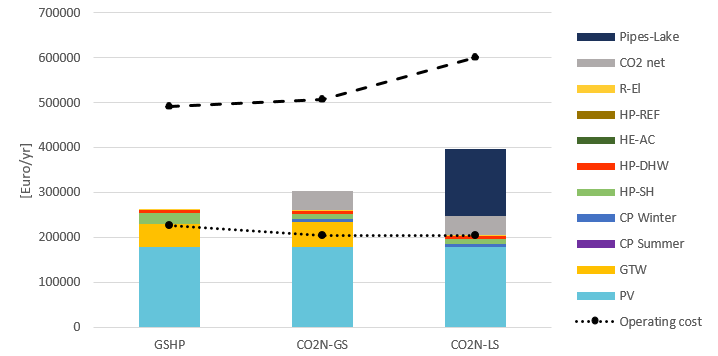
\includegraphics[width=1\textwidth]{V_costs.PNG}
	\caption{Cost comparison for the three different energy systems variants}
	\label{fig:V_costs}
\end{figure}
\todo{no TC in legend}
\todo{take out LS?}
\todo{add exergy values}
\todo{autarchy and autoconsumption values?}

OC of lake are slightly lower than CO2 geoth, even if tevap lower, since its a R1234yf HP with higher efficiencies... \\

Table \ref{tab:V_cops}.
\todo{graph with COP_t from JPNB}

\begin{table}[htp]
\centering
\caption{COP values for the three energy system}\vspace{2mm}
\label{tab:V_cops} 
\begin{tabular}{lrrr}
	\toprule
	& GS-HP & GS-CO2DEN & LS-CO2DEN \\ \midrule
	HP-SH            & 4.5  & 10.8    & 10.8    \\
	HP-DHW           & 3.8  & 6.2     & 6.2     \\
	HP-REF           & 5.4  & 8.1     & 8.1     \\
	HP-$CP_{winter}$ & -    & 15.8    & 12.6    \\
	Heating          & 4.0  & 5.2     & 4.9     \\
	Cooling          & 19.1 & 50.4      & 50.4      \\
	Global           & 4.6  & 6.1     & 5.6    \\ \bottomrule
\end{tabular}
\end{table}



\subsection{Ground temperature}
\begin{figure}[htp]
	\centering
	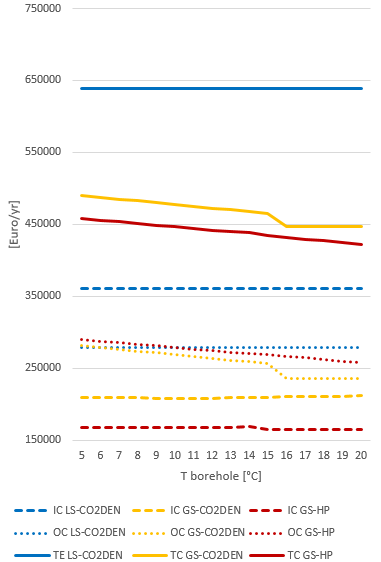
\includegraphics[width=0.45\textwidth]{V_SA_Tg.png}
	\caption{Cost comparison of variants in function of the borehole temperature}
	\label{fig:V_SA_Tg}
\end{figure}
\todo{wrapfigure}

%\begin{wrapfigure}{R}{0.5\textwidth} 
%	\vspace{-20pt}
%	\centering
%	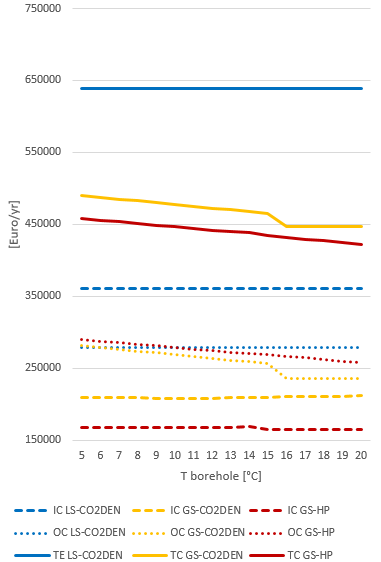
\includegraphics[width=0.45\textwidth]{V_SA_Tg.png}
%	\caption{Cost comparison of variants in function of the borehole temperature}
%	\label{fig:V_SA_Tg}
%	\vspace{-20pt}
%\end{wrapfigure}

A critical parameter for the efficiency of a ground sourced energy system is the ground temperature. As seen in Section \ref{ss:gtw}, this temperature depends mainly on the depth, the temperature gradient in the given soil and the surface temperature. In other words, it is dependent from the location - including local climate and altitude - and the depth of drilling. In order to aknowledge the influence this temperature has on the systems performance, a sensitivity analysis has been performed. The results are shown in Figure \ref{fig:V_SA_Tg}\\

The GS-HP energy system seems to responds in a linear way to the temperature raise. In reality a small step can be identified between 14 and 15 \si{\celsius}, at which the IC drop and the OC rise. This step happens when the ground is not cool enough anymore to profit from free-cooling. The system is forced to use a refrigeration system instead, which increases the OC. However this system is already installed and thus the increase if $IC_{HP-REF}$ is lower than the obsolete $IC_{HE-AC}$.\\

The GS-CO2DEN energy system presents a more evident step in its response to the ground temperature. The reason lies only in the use of the central plant. In fact, as described in Section \todo{write and reference model with if conditions}, if the soil has a $T_{b} \geq 16 \si{\celsius}$, the CP can source heat directly from the ground without the need of a heat pump, which drastically reduces the operational costs.\\

For obvious reason, while GS-CO2DEN and GSHP respond similarly to the variation in the bore temperature, the LS-CO2DEN presents constant costs. Despite not being dependent from the ground temperature, the system is represented on the graph for comparison. It can be seen that $OC_{LS-CO2DEN}$ is slightly higher than the other two energy systems for borehole temperatures above 10 \si{\celsius}. The lake distance in the Eglantine district is 1500m , which results in very high investment costs, which preclude the competitiveness of this solution, in the given conditions.\\


This would correspond to a geographical location, since ground has different temperatures in different latitudes and countries.

In Switzerland this would correspond to different well depth. To study this thoroughly it would be necessary to have a model for the geothermal well, taking into account the temperature gradient in function of depth, as well as the varying heat transfer coefficient for the CO2 vapor on the upward pipe. This model should also account for the recharge rate of the soil, which would improve the equipment sizing.

Assuming uniform soil, to maintain a constant heat capacity, a higher borehole temperature mean deeper wells, in a smaller number (maintain total meters).


\subsection{Lake distance}
Lake presents a lower average temperature than ground, but also smaller minimum approach temperature needed, but also higher compressor efficiency, given being a r1234yf hp. 

In comparison 7.5 - 4dTwater - 4dTminwr = -0.5 VS 15 - 6.8dTmingr = 8.2

Resulting in very similar but slightyl higher OC. The main advantage can be the reduction of upfront costs, by avoiding geothermal drilling. Pressure losses as well as the energy for pumping have been neglected, so the cost of the water pipes is mainly dependent on the distance of the lake water. Thus the threshold for the distance of the lake can be calculated, for which the LS-CO2DEN system to present a lower total cost than the GS-CO2DEN system. 

A sensitivity analysis has been performed on this threshold, in function of the ground temperature. The resulting thresholds are plotted on Figure \ref{fig:lakeDist}. This helps choosing between using the lake or the soil as a heat source, knowing the mean ground temperature and the distance from the lake water.

\begin{figure}[htp]
	\centering
	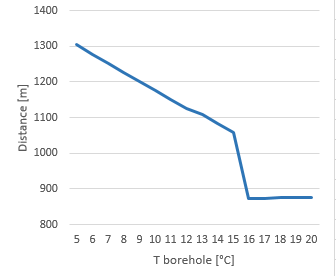
\includegraphics[width=0.45\textwidth]{lakeDist.png}
	\caption{Maximum distance of lake for which the total costs are lower than the two other energy systems, in function of the ground temperature $T_{borehole}$}
	\label{fig:lakeDist}
\end{figure}
\todo{wrapfig}

At $T_{borehole} = 12 \si{\celsius}$, as in the Eglantine district, the LS-CO2DEN would be a financially interesting solution against  GS-HP and GS-CO2DEN if the distance to the lake is respectively shorter than 257 and 563 meters.


\subsection{Optimization of energy demand}
The Eglantine district is for 97\% of residential use (see Section \ref{ss:Eglantine}), resulting in a very low cooling and refrigeration demand. It is now legitimate to wonder how the different energy systems would perform in a different district, i.e. with a different building use and thus a differently composed energy demand. With this aim in mind, it is also interesting to find out the optimum district composition for the performance of a CO2DEN system.\\

As per Table \ref{tab:ppa_buildinguse}, the building categories are:
\begin{enumerate}
	\item Housing (Multidwelling)
	\item Retail
	\item Restaurant services
	\item Indoor swimming pool
\end{enumerate}
For sake of simplicity, among the categories shown in Table \ref{tab:ppa_buildinguse}, the two most common and diverse - i.e. presenting the most different energy demand - have been chosen: (1) Housing and (2) Retail. 

A sensitivity analysis has been performed on a district composed by those two categories. The energy demand resulting from the different combinations of the above mentioned categories is shown in Figure \ref{fig:CU_E}. It is clear to see that the Retail building has a high cooling demand during summer months, with demand peaks that are around 4 times the heating demand peaks. Moreover, while the space heating demand remains very similar, the hot water demand decreases considerably.

\begin{figure}[htp]
	\centering
	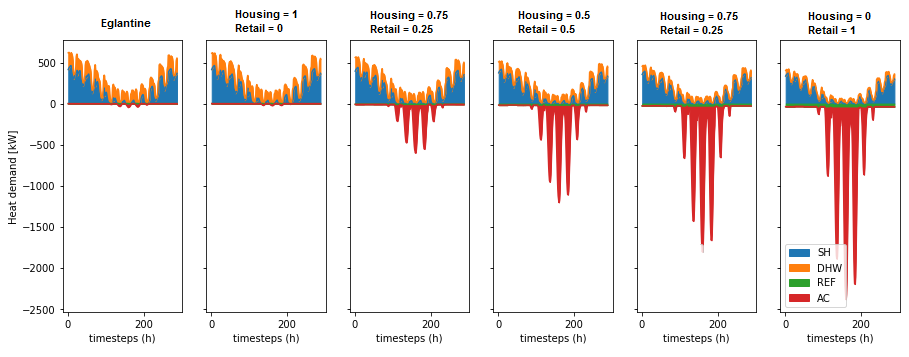
\includegraphics[width=1\textwidth]{CU_Edemand.png}
	\caption{Comparison of the energy demand (power) for the different use of buildings throughout the year}
	\label{fig:CU_E}
\end{figure}

\begin{figure}[htp]
	\centering
	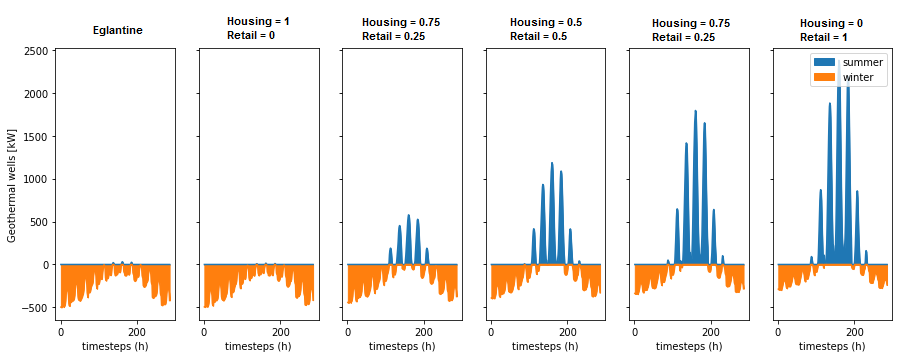
\includegraphics[width=1\textwidth]{CU_gtw.png}
	\caption{Comparison of the energy demand (power) of heat extracted (WINTER) of injected (SUMMER) into the boreholes}
	\label{fig:CU_gtw}
\end{figure}
\todo{needed figure of source?}

The resulting costs are shown in Figures \ref{fig:CU_TC}. 
%\begin{figure}[!htb]
%	\centering
%	\begin{minipage}{.45\textwidth}
%		\centering
%		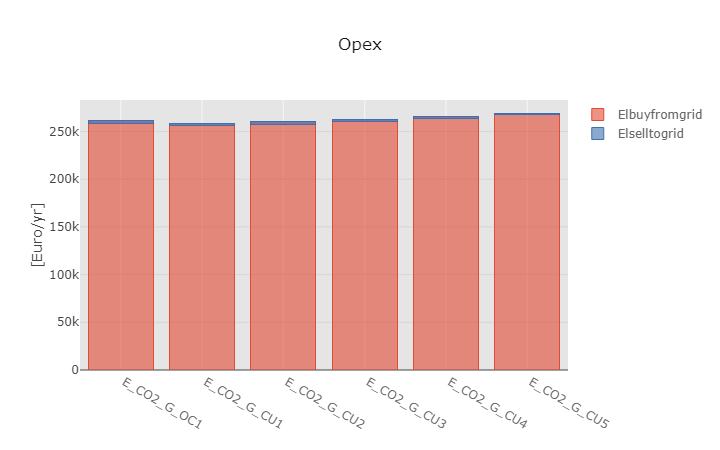
\includegraphics[width=\textwidth]{CU_OC.png}
%		\caption{Operating  cost for each combination of buildings use}
%		\label{fig:CU_OC}	
%	\end{minipage}%
%	\hspace{1cm}
%	\begin{minipage}{0.45\textwidth}
%		\centering
%		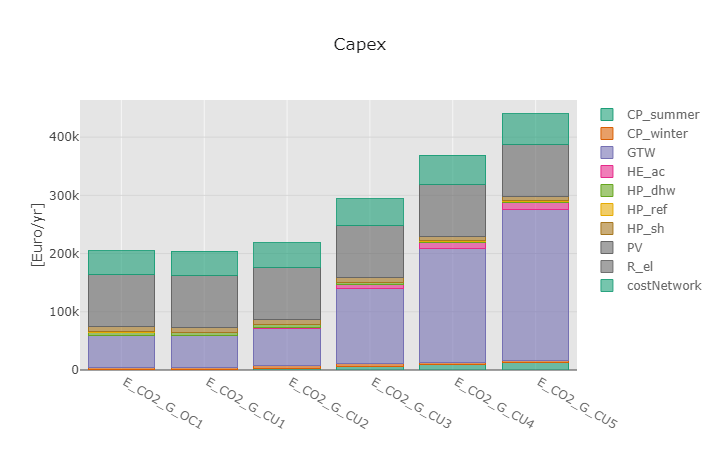
\includegraphics[width=\textwidth]{CU_IC.png}
%		\caption{Investment cost for each combination of buildings use}
%		\label{fig:CU_IC}
%	\end{minipage}
%\end{figure}

\begin{figure}[htp]
	\centering
	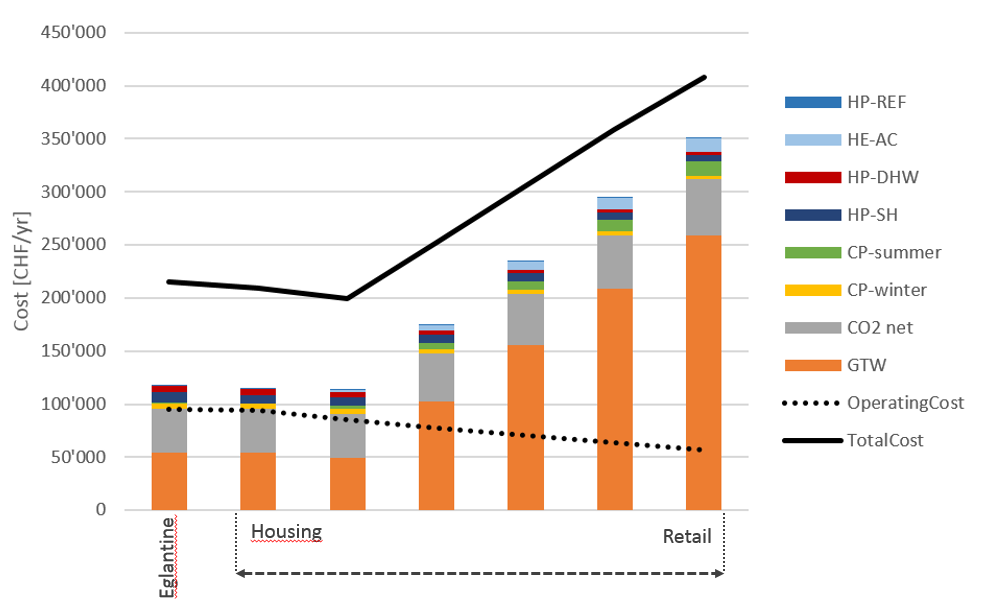
\includegraphics[width=0.75\textwidth]{CU_SA_TC.png}
	\caption{Cost comparison for different combinations of \textit{housing} and \textit{retail} building use, with the Eglantine district as a reference in the first column. The stacked columns show the investment costs.}
	\label{fig:CU_TC}
\end{figure}

Almost no difference in OC, Figure \ref{fig:CU_OC}.
There is no reason to lower OP since its about free cooling more than refrigeration. The only way if they happened in the same moment, since model does not account for heat storage in GTW.\\

The IC are strongly dependent on GTW cost. These are modeled in function of the peak demand. Thus given the very high cooling peaks originated by retail, the sizing of the gtw increases accordingly, what drastically increases the IC of the system. \\\\


\begin{figure}[tph]
	\centering
	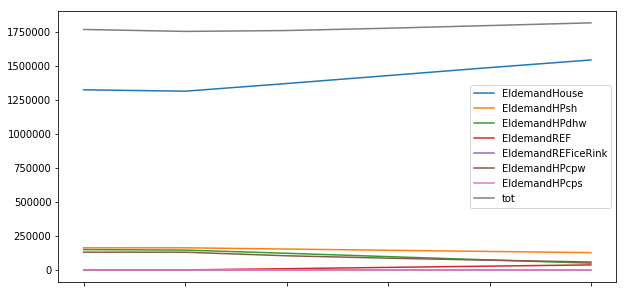
\includegraphics[width=0.45\linewidth]{Images/CU_el}
	\caption{Electricity demand in function of the building use composition}
	\label{fig:CU_el}
\end{figure}
\todo{wrapfig}

But what is the optimum combination?

To answer this questions, a model has been implemented that lets the solver choose the composition of the district. This requires an additional set of constraints, which ensures that the chosen composition is maintained throughout all the timesteps:
\begin{equation}
f_{h,t} = f_{h,t+1} \ \forall \ t \in T, \ h \in H
\end{equation}
where $f_{h,t}$ is the sizing variable of unit h in timestep t (see Section \ref{ss:osmose}) and H is a subset of units U, corresponding to the above mentioned building categories.

Every unit h in H has been sized to the total ERA of the Eglantine district. Thus, in order to have comparable results, the next constraint ensures that the share of all h sum up to the size of the Eglantine district:
\begin{equation}
\sum_{h}^{H} f_{h,t} = 1 \ \forall \ t \in T, \ h \in H
\end{equation}

The combination presenting lowest operating cost is found to be at:
$$f_{Retail} = 0.134$$
$$f_{Housing} = 0.866$$


\subsubsection{Ground/CU}

\begin{figure}[!htb]
	\centering
	\begin{minipage}{.45\textwidth}
		\centering
		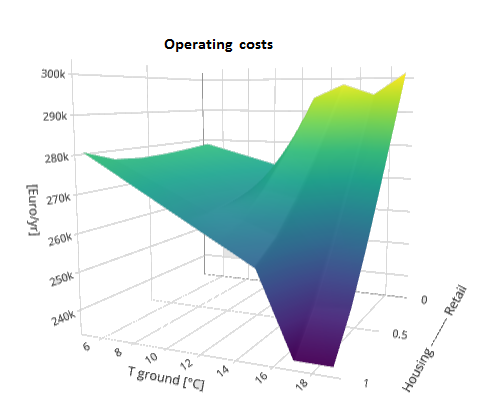
\includegraphics[width=\textwidth]{SA_CU_Tg_OC_py.png}
		\caption{Operating costs in function of the borehole temperature and the building use in the district}
		\label{fig:CU_Tg_OC}
	\end{minipage}%
	\hspace{1cm}
	\begin{minipage}{0.45\textwidth}
		\centering
		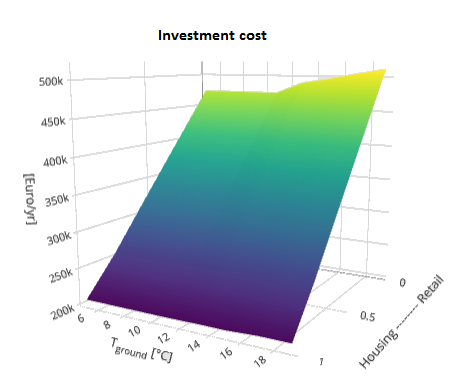
\includegraphics[width=\textwidth]{SA_CU_Tg_IC_py.png}
		\caption{Investment costs in function of the borehole temperature and the building use in the district}
		\label{fig:CU_Tg_IC}
	\end{minipage}
\end{figure}



\subsection{External heat source}
The integration of external heat sources, big as for example the ice rink in Eglantine case, is very interesting for this technology. However, this always depends on the ratio between the IC and the OC. In this case, this can be calculated with the ratio between the additional meters of pipes that have to be installed, wrt the amount of heat that can be recovered per year.
\todo{good thing to do?}


An new and efficient cooling system, together with an intelligent (weather, use, conditions...) management system, can drastically reduce energy consumption. This should be considered in the inclusion of the ice rink as heat source, since the renovation of the existing ice rink, or the construction of a new ice rink, would considerably reduce the amount of available waste heat.


%\subsection{CO2 network temperature control}
%An optimum for the temperature of the CO2 network has been defined \todo{missing ref}.
%The question arises if this temperature might vary in function of the operating condition of the network, i.e. the balance of heating and cooling load, the heat source temperature...\\
%A model has been implemented to study this, by leaving the optimizer choose the optimal operating temperature of the network for every given timestep.\\
%The results show that...
%\missingfigure{graph of $Temp_net(time)$}
%Then a simple representative scenario has been modeled, with a typical building, and a typical refrigeration, and varying \% of cooling load, wrt heating load.
%\missingfigure{graph of $Temp_net$(\% of cooling/heating)}


\section{Outlook}
This and this has been analyzed and results have shown.\\

However, it would be very interesting to make detailed analysis of...\\

This model should be improved...

The crucial aspect are geothermal wells, its sizing and thus its investment costs. For this a better model should be developed.

Geothermal model: In Switzerland this would correspond to different well depth. To study this thoroughly it would be necessary to have a model for the geothermal well, taking into account the temperature gradient in function of depth, as well as the varying heat transfer coefficient for the CO2 vapor on the upward pipe\cite{badacheExperimentalStudyCarbon2018,lamarcheReviewMethodsEvaluate2010}. This model should also account for the recharge rate of the soil, which would improve the equipment sizing. And thus storage, or gain through restoring/injecting heat.\\
Conductivity models \cite{jiaReviewEffectiveThermal2019,lamarcheReviewMethodsEvaluate2010,zengHeatTransferAnalysis2003a}
This new thing could be integrated...\\

\section{Conclusion}


%%%%%%%%% References %%%%%%%%%
\clearpage
\bibliographystyle{unsrt} %other styles: https://www.sharelatex.com/learn/Bibtex_bibliography_styles
\bibliography{bibliography.bib}

%%%%%%%%% Appendices %%%%%%%%%
\clearpage
\section{Anergy nets Switzerland}
\label{as:anergy_suisse}
\begin{landscape}
\begin{table}[h]
\centering
\caption{District energy systems in Switzerland ~\cite{energieschweizFallbeispieleThermischeNetze2018}; \textit{n/a}: not available}\vspace{2mm} 
\label{tab:anergieCH1} 
\begin{tabular}{llllllll}
\toprule
                                                                               & \textbf{\begin{tabular}[c]{@{}l@{}}Anergienetz \\ ETH \\ Hönggerberg\end{tabular}} & \textbf{\begin{tabular}[c]{@{}l@{}}Jardins de \\ la Pâla\end{tabular}}      & \textbf{\begin{tabular}[c]{@{}l@{}}Suurstoffi-\\ Areal\end{tabular}}                                  & \textbf{\begin{tabular}[c]{@{}l@{}}Anergienetz \\ Friesenberg (FGZ)\end{tabular}} & \textbf{\begin{tabular}[c]{@{}l@{}}CAD La-\\ Tour-De-Peilz\end{tabular}} & \textbf{\begin{tabular}[c]{@{}l@{}}Anergienetz-\\ Visp\end{tabular}}  & \textbf{\begin{tabular}[c]{@{}l@{}}Genève-Lac-\\ Nations (GLN)\end{tabular}}  \\
                                                                               \midrule
\textbf{Location}                                                              & Zürich                                                                             & Bulle                                                                       & Rotkreuz                                                                                              & Zürich                                                                            & La-Tour-de-Peilz                                                         & Visp                                                                  & Genève                                                                        \\
\textbf{Year of construction}                                                  & 2012 - 2026                                                                        & 2012 - 2020                                                                 & 2010 - 2020                                                                                           & 2011-2050                                                                         & 2013 - 2015                                                              & 2007 - heute                                                          & 2008 - 2016                                                                   \\
\textbf{Type}                                                                  & $\leq$ 20 \si{\celsius}                                                                            & $\leq$ 20 \si{\celsius}                                                                     & $\leq$ 20 \si{\celsius}                                                                                               & $\leq$ 20 \si{\celsius}                                                                           & $\leq$ 20\si{\celsius}                                                                   & $\leq$ 20 \si{\celsius}                                                               & $\leq$ 20 \si{\celsius}                                                                       \\
\textbf{Energy Ref. Area $[m2]$}                                                              & 475'000                                                                            & 65‘000                                                                      & 172'421                                                                                               & 185'000                                                                           & 24 Buildings                                                             & 160'000                                                               & 840'000                                                                       \\
\textbf{Use}                                                                   & \begin{tabular}[c]{@{}l@{}}School\\ Residential\end{tabular}                       & \begin{tabular}[c]{@{}l@{}}Residential\\ Commercial\\ Industry\end{tabular} & \begin{tabular}[c]{@{}l@{}}Residential\\ Administration\\ Commercial\\ Catering\\ School\end{tabular} & \begin{tabular}[c]{@{}l@{}}Residential\\ Computation\end{tabular}                 & \begin{tabular}[c]{@{}l@{}}Residential\\ Administration\end{tabular}     & \begin{tabular}[c]{@{}l@{}}Residential\\ Industry\end{tabular}        & \begin{tabular}[c]{@{}l@{}}Residential\\ Administration\\ School\end{tabular} \\
\textbf{Status}                                                                & Partly built                                                                       & Partly built                                                                & Partly built                                                                                          & Partly built                                                                      & Built                                                                    & Built                                                                 & Built                                                                         \\
\midrule
\textbf{}                                                                      & \multicolumn{7}{c}{Data Energy Consumption}                                                                                                                                                                                                                                                                                                                                                                                                                                                                                                                                                     \\
\midrule
\textbf{\begin{tabular}[c]{@{}l@{}}Inst. Heating\\ capacity $[kW]$\end{tabular}} & 8'000                                                                              & 2'000                                                                       & 6'732                                                                                                 & 3'930                                                                             & 10'000                                                                   & 3'467                                                                 & 4'300                                                                         \\
\textbf{\begin{tabular}[c]{@{}l@{}}Heating demand \\ $[MWh/a]$\end{tabular}}   & 28'450                                                                             & 3'100                                                                       & 10'619                                                                                                & 35'000                                                                            & 812                                                                      & 8'737                                                                 & 5’000                                                                         \\
\textbf{\begin{tabular}[c]{@{}l@{}}Inst. Cooling\\ capacity $[kW]$\end{tabular}} & 6'000                                                                              & 1'000                                                                       & 2'327                                                                                                 & 3'500                                                                             & None                                                                     & 2'600                                                                 & 16'200                                                                        \\
\textbf{\begin{tabular}[c]{@{}l@{}}Cooling demand \\ $[MWh/a]$\end{tabular}}   & 26'200                                                                             & 650                                                                         & 2'364                                                                                                 & 80'000                                                                            & None                                                                     & 3'380                                                                 & 20'000                                                                        \\
\textbf{Heat source}                                                           & \begin{tabular}[c]{@{}l@{}}Laboratories\\ waste heat \\ +HP\end{tabular}           & Groundwater+HP                                                              & \begin{tabular}[c]{@{}l@{}}Waste heat \\ buildings \\ + PVT (solar th.) \\ +HP\end{tabular}           & \begin{tabular}[c]{@{}l@{}}Waste heat\\ data center+HP\end{tabular}               & Lake water +HP                                                           & \begin{tabular}[c]{@{}l@{}}Inudstrial waste \\ heat + HP\end{tabular} & Lake water +HP                                                                \\
\textbf{Heat storage}                                                          & \begin{tabular}[c]{@{}l@{}}Geothermal well \\ field\\ (431 at 200m)\end{tabular}   & Groundwater 12\si{\celsius}                                                            & \begin{tabular}[c]{@{}l@{}}Geothermal well\\ field \\ (215 at 150 m,\\ 180 at 280m)\end{tabular}      & \begin{tabular}[c]{@{}l@{}}Geothermal well\\ field\\ (332 at 250m)\end{tabular}   & None                                                                     & None                                                                  & None                                                                          \\
\midrule
\textbf{}                                                                      & \multicolumn{7}{c}{Network data}                                                                                                                                                                                                                                                                                                                                                                                                                                                                                                                                                                \\
\midrule
\textbf{Network length $[km]$}                                                   & 1.5                                                                                & 0.85                                                                        & 2.5                                                                                                   & 1.5                                                                               & 4.1                                                                      & 4.2                                                                   & 6                                                                             \\
\textbf{Heating pipeT}                                                         & 24 \si{\celsius} - 8 \si{\celsius}                                                                       & 12 \si{\celsius} - 9 \si{\celsius}                                                                & 25 \si{\celsius} - 8 \si{\celsius}                                                                                          & 28 \si{\celsius} - 8 \si{\celsius}                                                                      & 20 \si{\celsius} - 6 \si{\celsius}                                                             & 18 \si{\celsius} - 8 \si{\celsius}                                                          & 17 \si{\celsius} - 5 \si{\celsius}                                                                  \\
\textbf{Cooling pipeT}                                                         & 4 \si{\celsius} - 20 \si{\celsius}                                                                       & 4 \si{\celsius} - 17 \si{\celsius}                                                                & 4 \si{\celsius} - 17 \si{\celsius}                                                                                          & 4 \si{\celsius} -24 \si{\celsius}                                                                       & 2 \si{\celsius} - 16 \si{\celsius}                                                             & 4 \si{\celsius} - 16 \si{\celsius}                                                          & 5 \si{\celsius} - 12 \si{\celsius}                                                                  \\
\textbf{Pipe diameter $[mm]$}                                                    & DN 560                                                                             & 75 - 250                                                                    & 60 - 400                                                                                              & 400 - 500                                                                         & 400 -700                                                                 & DN 400                                                                & 100 -700                                                                      \\
\textbf{Number of pipes}                                                       & 3                                                                                  & 2                                                                           & 2                                                                                                     & 2                                                                                 & 2                                                                        & 2                                                                     & 2       \\
\bottomrule
\end{tabular}
\end{table}

\end{landscape}
\begin{landscape}
\begin{table}[h]
\centering
\caption{District energy systems in Switzerland}\vspace{2mm}
\label{tab:anergieCH2} 
\begin{tabular}{llllllll}
\toprule

                                                                                      & \textbf{\begin{tabular}[c]{@{}l@{}}Anergienetz \\ ETH \\ Hönggerberg\end{tabular}} & \textbf{\begin{tabular}[c]{@{}l@{}}Jardins de \\ la Pâla\end{tabular}}             & \textbf{\begin{tabular}[c]{@{}l@{}}Suurstoffi-\\ Areal\end{tabular}} & \textbf{\begin{tabular}[c]{@{}l@{}}Anergienetz \\ Friesenberg (FGZ)\end{tabular}} & \textbf{\begin{tabular}[c]{@{}l@{}}CAD La-\\ Tour-De-Peilz\end{tabular}}      & \textbf{\begin{tabular}[c]{@{}l@{}}Anergienetz-\\ Visp\end{tabular}} & \textbf{\begin{tabular}[c]{@{}l@{}}Genève-Lac-\\ Nations (GLN)\end{tabular}} \\
                                                                                      \midrule
\textbf{}                                                                             & \multicolumn{7}{c}{Financial data}                                                                                                                                                                                                                                                                                                                                                                                                                                                                                                                                       \\
\midrule
\textbf{\begin{tabular}[c]{@{}l@{}}Tot. investments\\ '[Mio.CHF]'\end{tabular}}       & 37                                                                                 & 6                                                                                  & n/a                                                                  & 42.5                                                                              & 32                                                                            & 1.26                                                                 & 33                                                                           \\
\textbf{Interest rate[\%]}                                                            & 3.9 - 6.7                                                                          &                                                                                    & n/a                                                                  & n/a                                                                               & 6.4                                                                           & 5.8 - 8                                                              & n/a                                                                          \\
\textbf{Lifespan [a]}                                                                 &                                                                                    &                                                                                    &                                                                      &                                                                                   &                                                                               &                                                                      &                                                                              \\
\textbf{Pipes}                                                                        & 50                                                                                 & 30                                                                                 & 40                                                                   & 50                                                                                & 50                                                                            & 40                                                                   & n/a                                                                          \\
\textbf{Storage}                                                                      & 50                                                                                 & None                                                                               & 80                                                                   & 50                                                                                & None                                                                          & None                                                                 & n/a                                                                          \\
\textbf{Heating unit}                                                                 & 20                                                                                 & 15                                                                                 & 20                                                                   & 20                                                                                & 25                                                                            & 20                                                                   & n/a                                                                          \\
\textbf{Cooling unit}                                                                 & 20                                                                                 & 15                                                                                 & 20                                                                   & 20                                                                                & 25                                                                            & 20                                                                   & n/a                                                                          \\
\textbf{\begin{tabular}[c]{@{}l@{}}Cost of energy \\ '[Rp./kWh]'\end{tabular}}        & \begin{tabular}[c]{@{}l@{}}7.7 \\ (Heating +cooling)\end{tabular}                  & \begin{tabular}[c]{@{}l@{}}5.85 – 8\\ (at the moment \\ only heating)\end{tabular} & n/a                                                                  & \begin{tabular}[c]{@{}l@{}}18\\ (Heating)\end{tabular}                            & \begin{tabular}[c]{@{}l@{}}19.8\\ (at the moment\\ only heating)\end{tabular} & \begin{tabular}[c]{@{}l@{}}22.9\\ (Heating +\\ cooling)\end{tabular} & n/a                                                                          \\
\textbf{Tot. COP of heating}                                                          & 7.2                                                                                & 4.4                                                                                & n/a                                                                  & 5.2                                                                               & n/a                                                                           & n/a                                                                  & n/a                                                                          \\
\textbf{\begin{tabular}[c]{@{}l@{}}Tot. COP of heating\\ (incl. Pumps…)\end{tabular}} & 5.8                                                                                & 2.7                                                                                & 2.7                                                                  & 4.1                                                                               & 3.5-4                                                                         & 4                                                                    & 6.5                                                                          \\
\textbf{Tot. EER of cooling}                                                          & 30.1                                                                               & n/a                                                                                & n/a                                                                  & n/a                                                                               & n/a                                                                           & n/a                                                                  & n/a                                                                          \\
\textbf{\begin{tabular}[c]{@{}l@{}}Tot. EER of cooling\\ (incl. Pumps…)\end{tabular}} & 6.9                                                                                & 12.1                                                                               & n/a                                                                  & n/a                                                                               & n/a                                                                           & n/a                                                                  & n/a \\
\bottomrule
\end{tabular}
\end{table}

\end{landscape}


%%%%%%%%%%%%%%%%%%%%%%%%%%%% END %%%%%%%%%%%%%%%%%%%%%%%%%%%%%%%%%%%
\end{document}
